\chapter{Оценка качества сварного соединения по сигналам коаксиальной фотодиодной системы}

\section{Постановка задачи}

В данной части работы исследованы экспериментальные данные, предоставленные научным руководителем. Данные были получены при лазерной сварке образцов из стали 09Г2С толщиной 4~мм с использованием системы оптического мониторинга \textit{ALPAS-WDD}. Эта система регистрирует излучение из зоны сварки по трём каналам: в видимом диапазоне, в канале отражённого лазерного излучения и в инфракрасном диапазоне. Такое разделение позволяет учитывать различные составляющие оптического отклика процесса: излучение плазменно-паровой области и парогазового канала, отражённую часть лазерного излучения, а также тепловое излучение нагретого металла и сварочной ванны.

Система \textit{ALPAS-WDD} предназначена для контроля процесса сварки и может самостоятельно использоваться для обнаружения дефектов сварного соединения. Однако для обучения её штатных алгоритмов требуется более 500 экспериментов. Получение такого количества сварных образцов и последующий контроль их качества являются крайне трудоемкой задачей. Поэтому в данной работе была поставлена более узкая задача: проверить, можно ли получить практически полезный результат при существенно меньшем объёме размеченных данных за счёт формирования оконных признаков и применения методов машинного обучения.

Предоставленная экспериментальная серия включала девять измерений: по три измерения для мощностей лазерного излучения 1.5, 2.0 и 3.5~кВт. Сварка выполнялась на лазерной системе ЛС-20 с использованием роботизированной системы перемещения Kuka KR120 и оптической схемы FLW D50. Диаметр оптического волокна составлял 200~мкм, фокусное расстояние коллиматора --- 160~мм, фокусное расстояние фокусирующей оптики --- 500~мм, диаметр пятна в фокусе --- 0.6~мм. Рассматривалось стыковое соединение.

Для каждого измерения была известна величина \(h_i\), характеризующая непровар. Согласно принятой постановке, значение \(h_i = 0\) соответствует отсутствию непровара, а \(h_i > 0\) --- наличию непровара, поскольку для изделий высокого качества непровар не допускается~\cite{gost_iso_13919_1_2025}.

Дальнейшая обработка данных направлена на проверку двух вопросов: возможно ли по сигналам фотодиодной системы качественно определить наличие непровара и возможно ли количественно оценить величину \(h_i\). Поскольку практическая задача связана с контролем процесса во время сварки, основной объект анализа был выбран в виде локального окна сигнала.

\section{Cтруктура экспериментальных данных}

Исходные данные были представлены в виде бинарных файлов, содержащих служебный заголовок и массив дискретных отсчётов. В начале файла записывалась длина заголовка, после чего следовал JSON-заголовок с основной информацией о записи. Оставшаяся часть файла интерпретировалась как массив целочисленных значений типа \texttt{int16}. После чтения данных выполнялось преобразование массива к форме, в которой строки соответствуют последовательным отсчётам, а столбцы --- отдельным каналам фотодиодной системы.

Достоверное значение частоты дискретизации для рассматриваемой серии измерений к не сохранилось. Поэтому дальнейшая обработка выполнялась во временной оси, выраженной в отсчётах. Вследствие этого временные координаты окон задавались номерами отсчётов, а частотные признаки рассматривались в относительных единицах дискретного спектра.

\section{Предварительная обработка сигналов}

Особенностью экспериментальных записей является то, что регистрация фотодиодных сигналов начинается до включения лазерного излучения и продолжается после его выключения. Вследствие этого исходные данные содержат неинформативные участки, соответствующие фоновому уровню до и после процесса сварки. Для дальнейшего анализа эти участки были исключены.

Определение активного участка выполнялось по каналу отражённого излучения. Такой выбор обусловлен тем, что данный канал демонстрировал наиболее устойчивое изменение уровня при включении лазерного излучения. Уровень фона оценивался по начальной и конечной частям записи, после чего определялись индексы, в которых сигнал отражённого излучения существенно превышал фоновое значение. Затем все три канала обрезались по одинаковым границам, что сохраняло синхронность сигналов.

На рис.~\ref{fig:photodiode_time_signals} приведён пример временных реализаций трёх каналов после удаления неинформативных участков. По оси абсцисс отложен номер отсчёта, по оси ординат --- значение сигнала в единицах АЦП.

\begin{figure}[H]
    \centering
    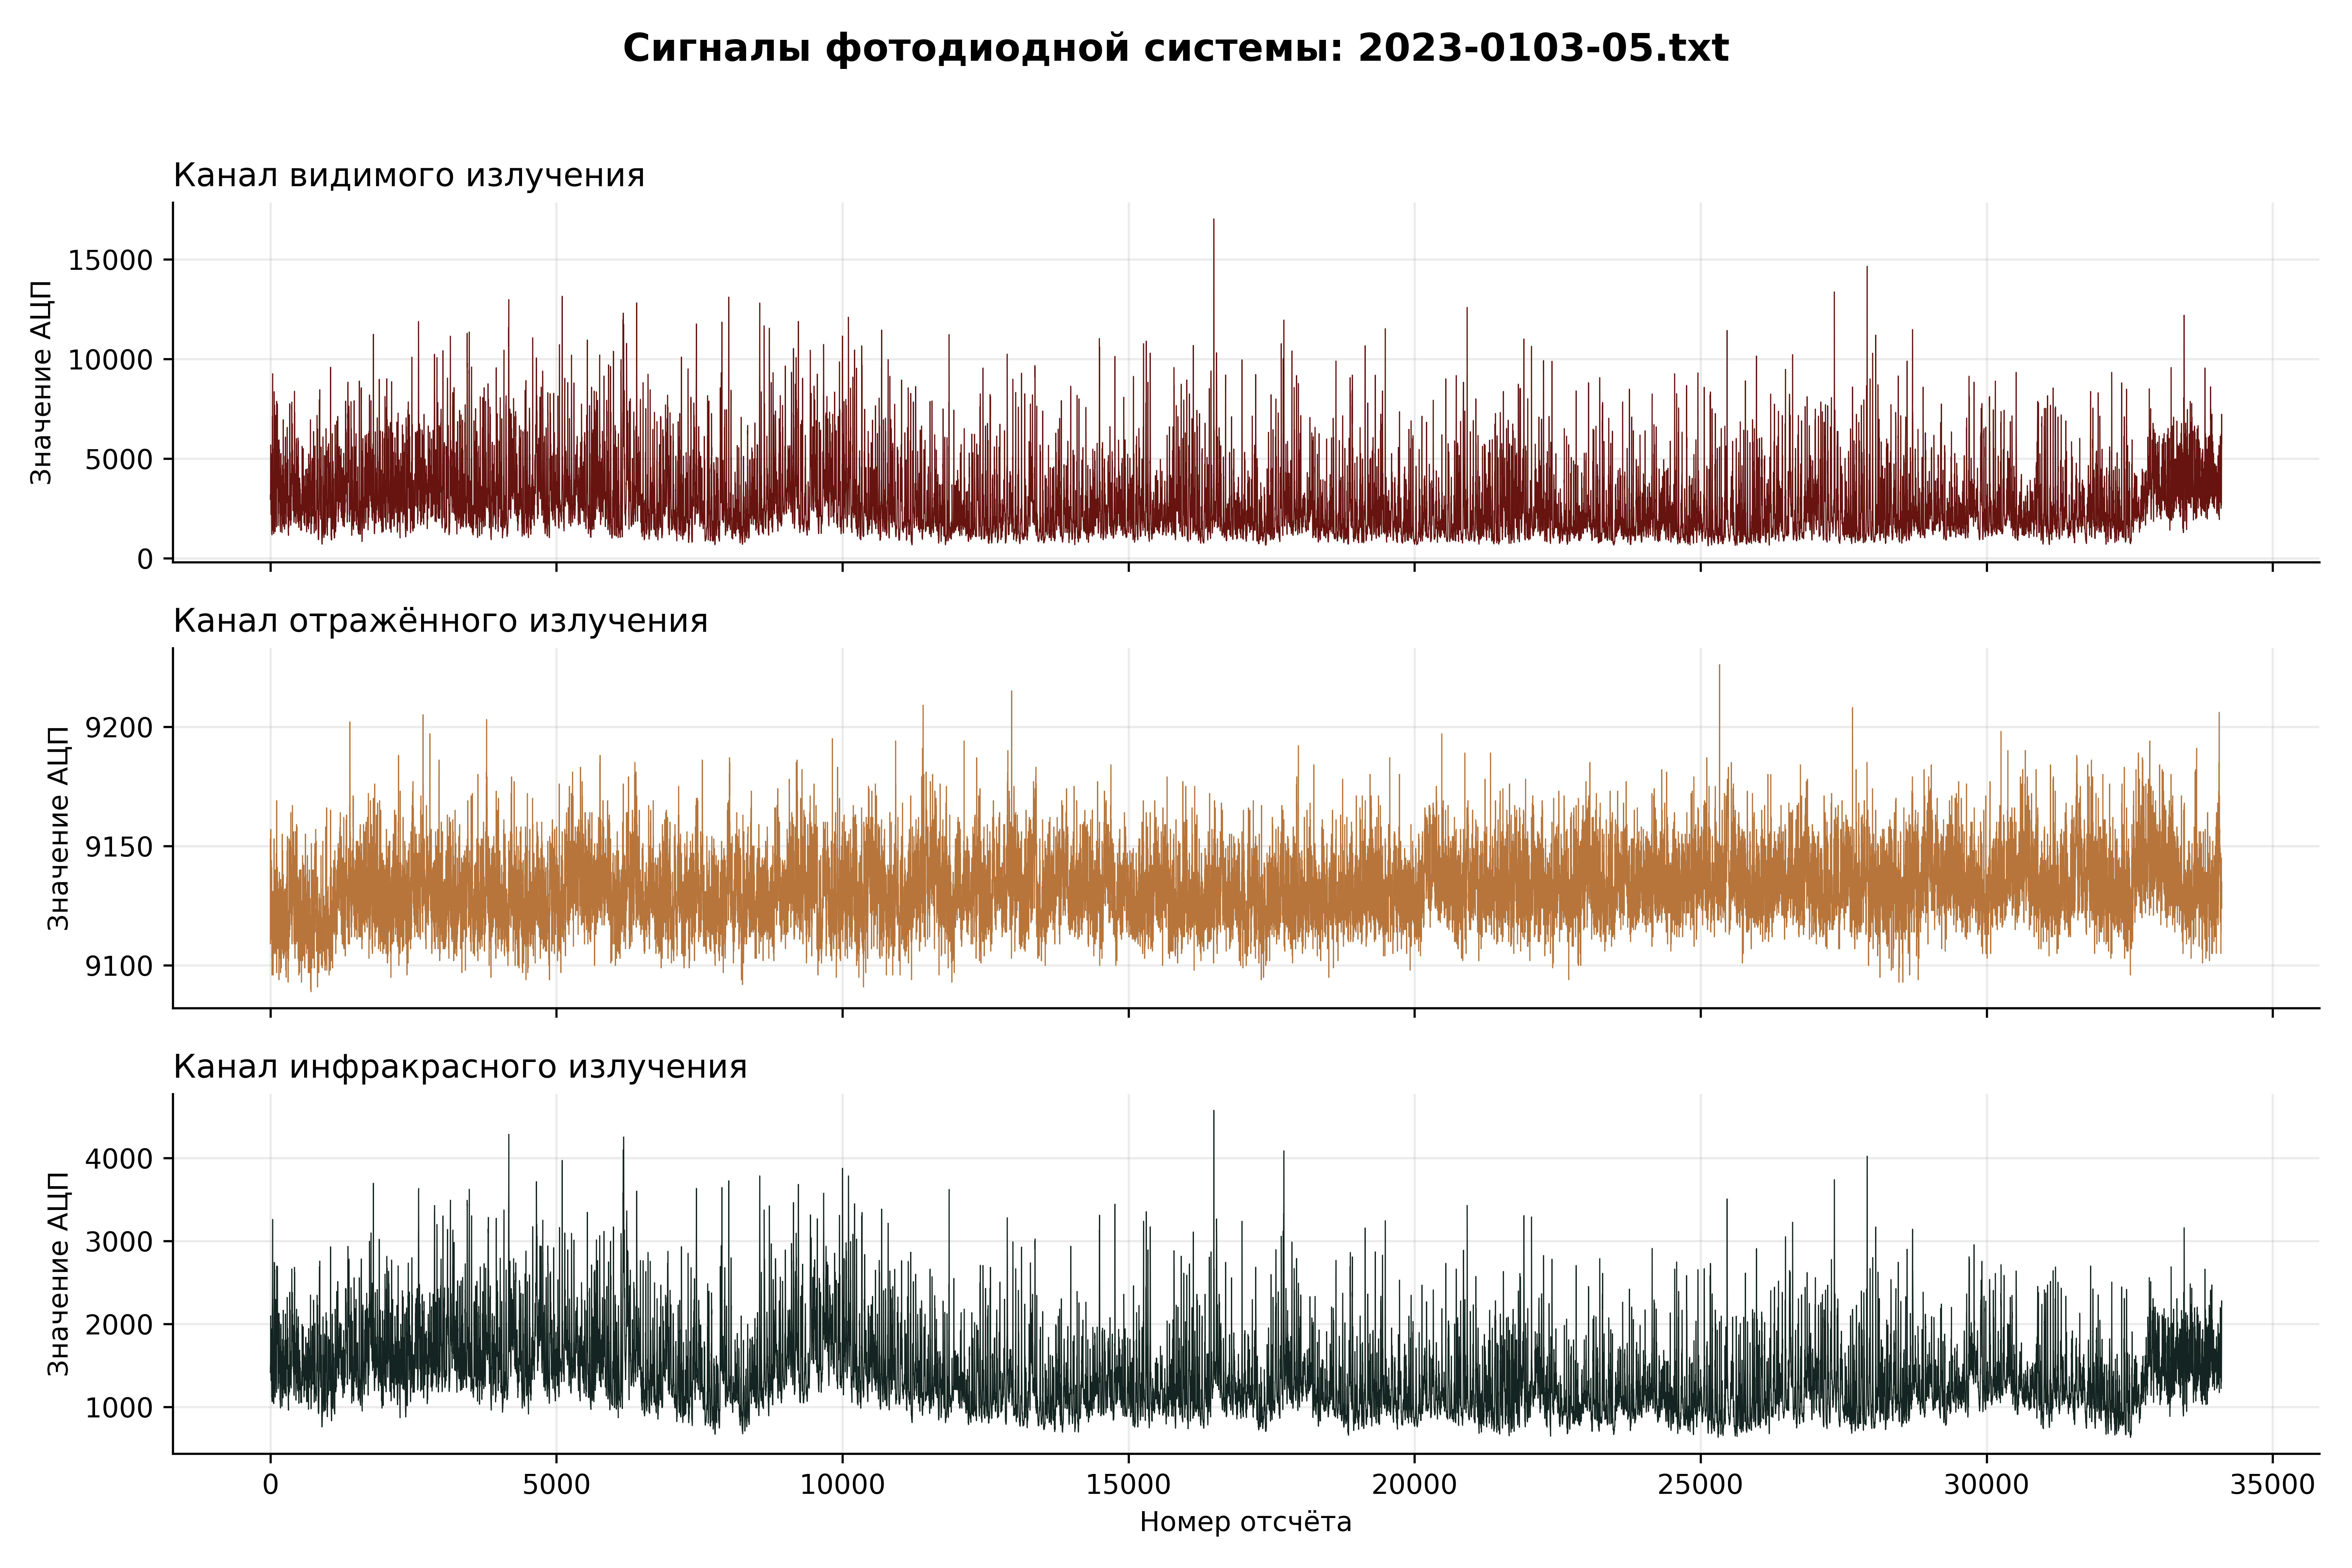
\includegraphics[width=0.95\textwidth]{figures/photodiode_time_signals.png}
    \caption{Пример зависимости значения АЦП сигналов коаксиальной фотодиодной системы от времени}
    \label{fig:photodiode_time_signals}
\end{figure}

После предварительной обработки каждый файл измерения содержал активный участок сигнала, соответствующий непосредственно процессу лазерной сварки. Далее этот участок разделялся на перекрывающиеся окна, поскольку задача работы связана не с анализом всего сварочного прохода после завершения процесса, а с оценкой качества в режиме, близком к реальному времени.

В качестве основного режима оконного анализа была выбрана длина окна 1500 отсчётов при шаге 750 отсчётов. Такое значение шага соответствует перекрытию соседних окон на 50~\%. Предварительный перебор различных длин окна показал, что как уменьшение, так и увеличение окна приводило к снижению качества классификации. Поэтому выбранный вариант рассматривался как компромисс между локальностью анализа и устойчивостью рассчитываемых признаков.

\section{Расчёт оконных признаков}

Для каждого окна рассчитывался набор признаков, описывающих поведение сигналов фотодиодной системы. Временные признаки характеризовали амплитудную структуру сигнала внутри окна. К ним относились среднее значение, стандартное отклонение, среднеквадратичное значение, минимум, максимум, размах, энергия, асимметрия, эксцесс, межквартильный размах, энтропия распределения амплитуд и число выраженных всплесков.

Кроме признаков отдельных каналов, рассчитывались межканальные признаки: отношения средних значений, отношения энергий и коэффициенты корреляции между каналами. Эти признаки позволяют учитывать не только абсолютный уровень сигнала в каждом канале, но и изменение баланса между различными составляющими оптического отклика процесса.

Дополнительно для каждого окна рассчитывались частотные признаки на основе быстрого преобразования Фурье. Перед вычислением спектра сигнал центрировался и нормировался на стандартное отклонение:
\[
    \tilde{x}_i = \frac{x_i - \bar{x}}{\sigma_x},
\]
где \(\bar{x}\) --- среднее значение сигнала в окне, \(\sigma_x\) --- стандартное отклонение. Такая нормировка уменьшает влияние абсолютного уровня сигнала и позволяет рассматривать относительную структуру флуктуаций.

По спектру каждого окна рассчитывались полная спектральная энергия, энергия в низкочастотной, среднечастотной и высокочастотной областях, отношение высокочастотной энергии к низкочастотной, доминирующая частота, спектральный центроид, максимальная амплитуда спектра, а также относительные доли энергии в частотных областях.

Спектральный центроид вычислялся как
\[
    f_c = \frac{\sum_{k} f_k P_k}{\sum_{k} P_k},
\]
где \(f_k\) --- частота \(k\)-й спектральной компоненты в относительных единицах дискретного спектра, \(P_k\) --- соответствующая спектральная мощность. Этот признак характеризует условный центр распределения энергии по частотам.

\section{Визуальная оценка разделимости окон}

На первом этапе была выполнена визуальная оценка разделимости окон, соответствующих отсутствию непровара и наличию непровара. Для этого строились диаграммы рассеяния для различных пар признаков. Каждая точка на таких диаграммах соответствует одному временному окну, а цвет точки задаёт класс качества сварного соединения.


На рис.~\ref{fig:defect_scatter_1} приведена диаграмма рассеяния для двух частотных признаков: относительной высокочастотной энергии видимого канала и спектрального центроида инфракрасного канала. Каждая точка соответствует одному временному окну, а цвет точки задаёт класс качества сварного соединения. Такая пара признаков позволяет одновременно учитывать изменение высокочастотной составляющей излучения в видимом диапазоне и смещение центра спектральной энергии в инфракрасном канале.

\begin{figure}[H]
    \centering
    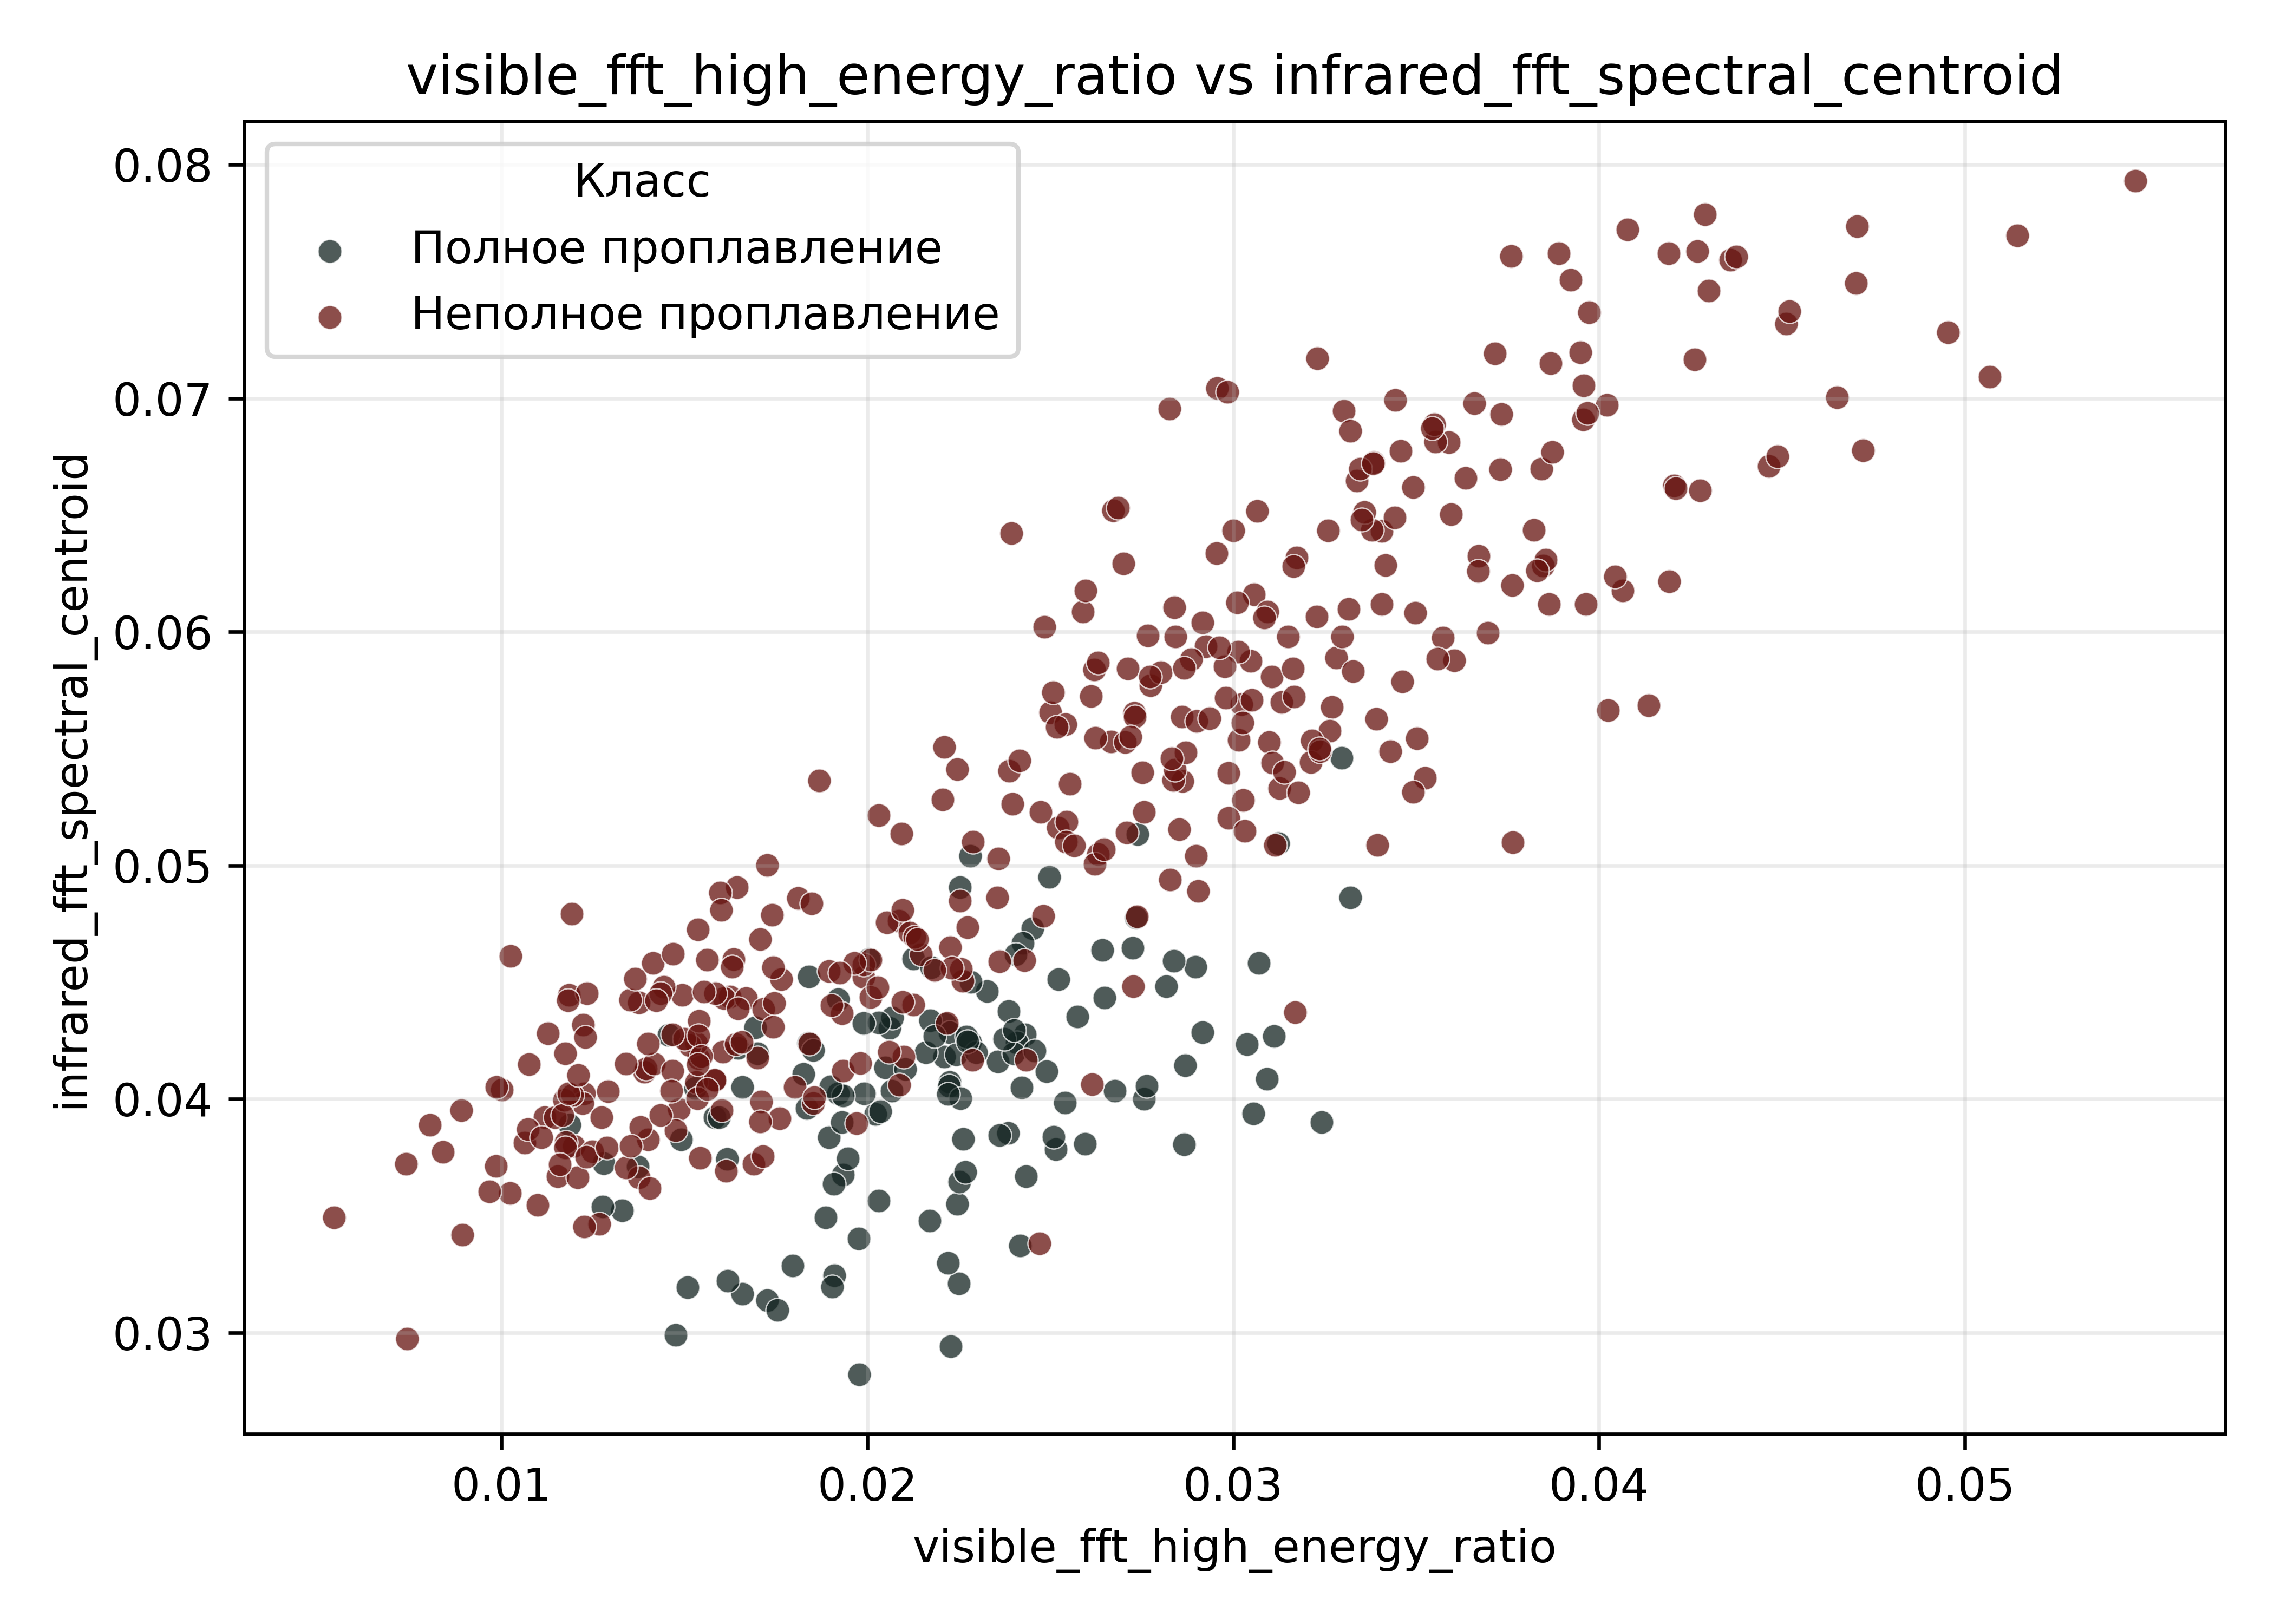
\includegraphics[width=0.78\textwidth]{figures/scatter_visible_fft_high_energy_ratio_vs_infrared_fft_spectral_centroid.png}
    \caption{Диаграмма рассеяния оконных частотных признаков: относительная высокочастотная энергия видимого канала и спектральный центроид инфракрасного канала}
    \label{fig:defect_scatter_1}
\end{figure}

На рис.~\ref{fig:defect_scatter_2} показана диаграмма рассеяния для двух временных признаков: стандартного отклонения инфракрасного канала и отношения среднего значения видимого канала к среднему значению инфракрасного канала. Первый признак характеризует амплитудную изменчивость инфракрасного сигнала в пределах окна, а второй отражает баланс между излучением в видимом и инфракрасном диапазонах. Такое сочетание признаков позволяет оценить, изменяется ли не только уровень отдельных каналов, но и соотношение между различными составляющими оптического отклика процесса.

\begin{figure}[H]
    \centering
    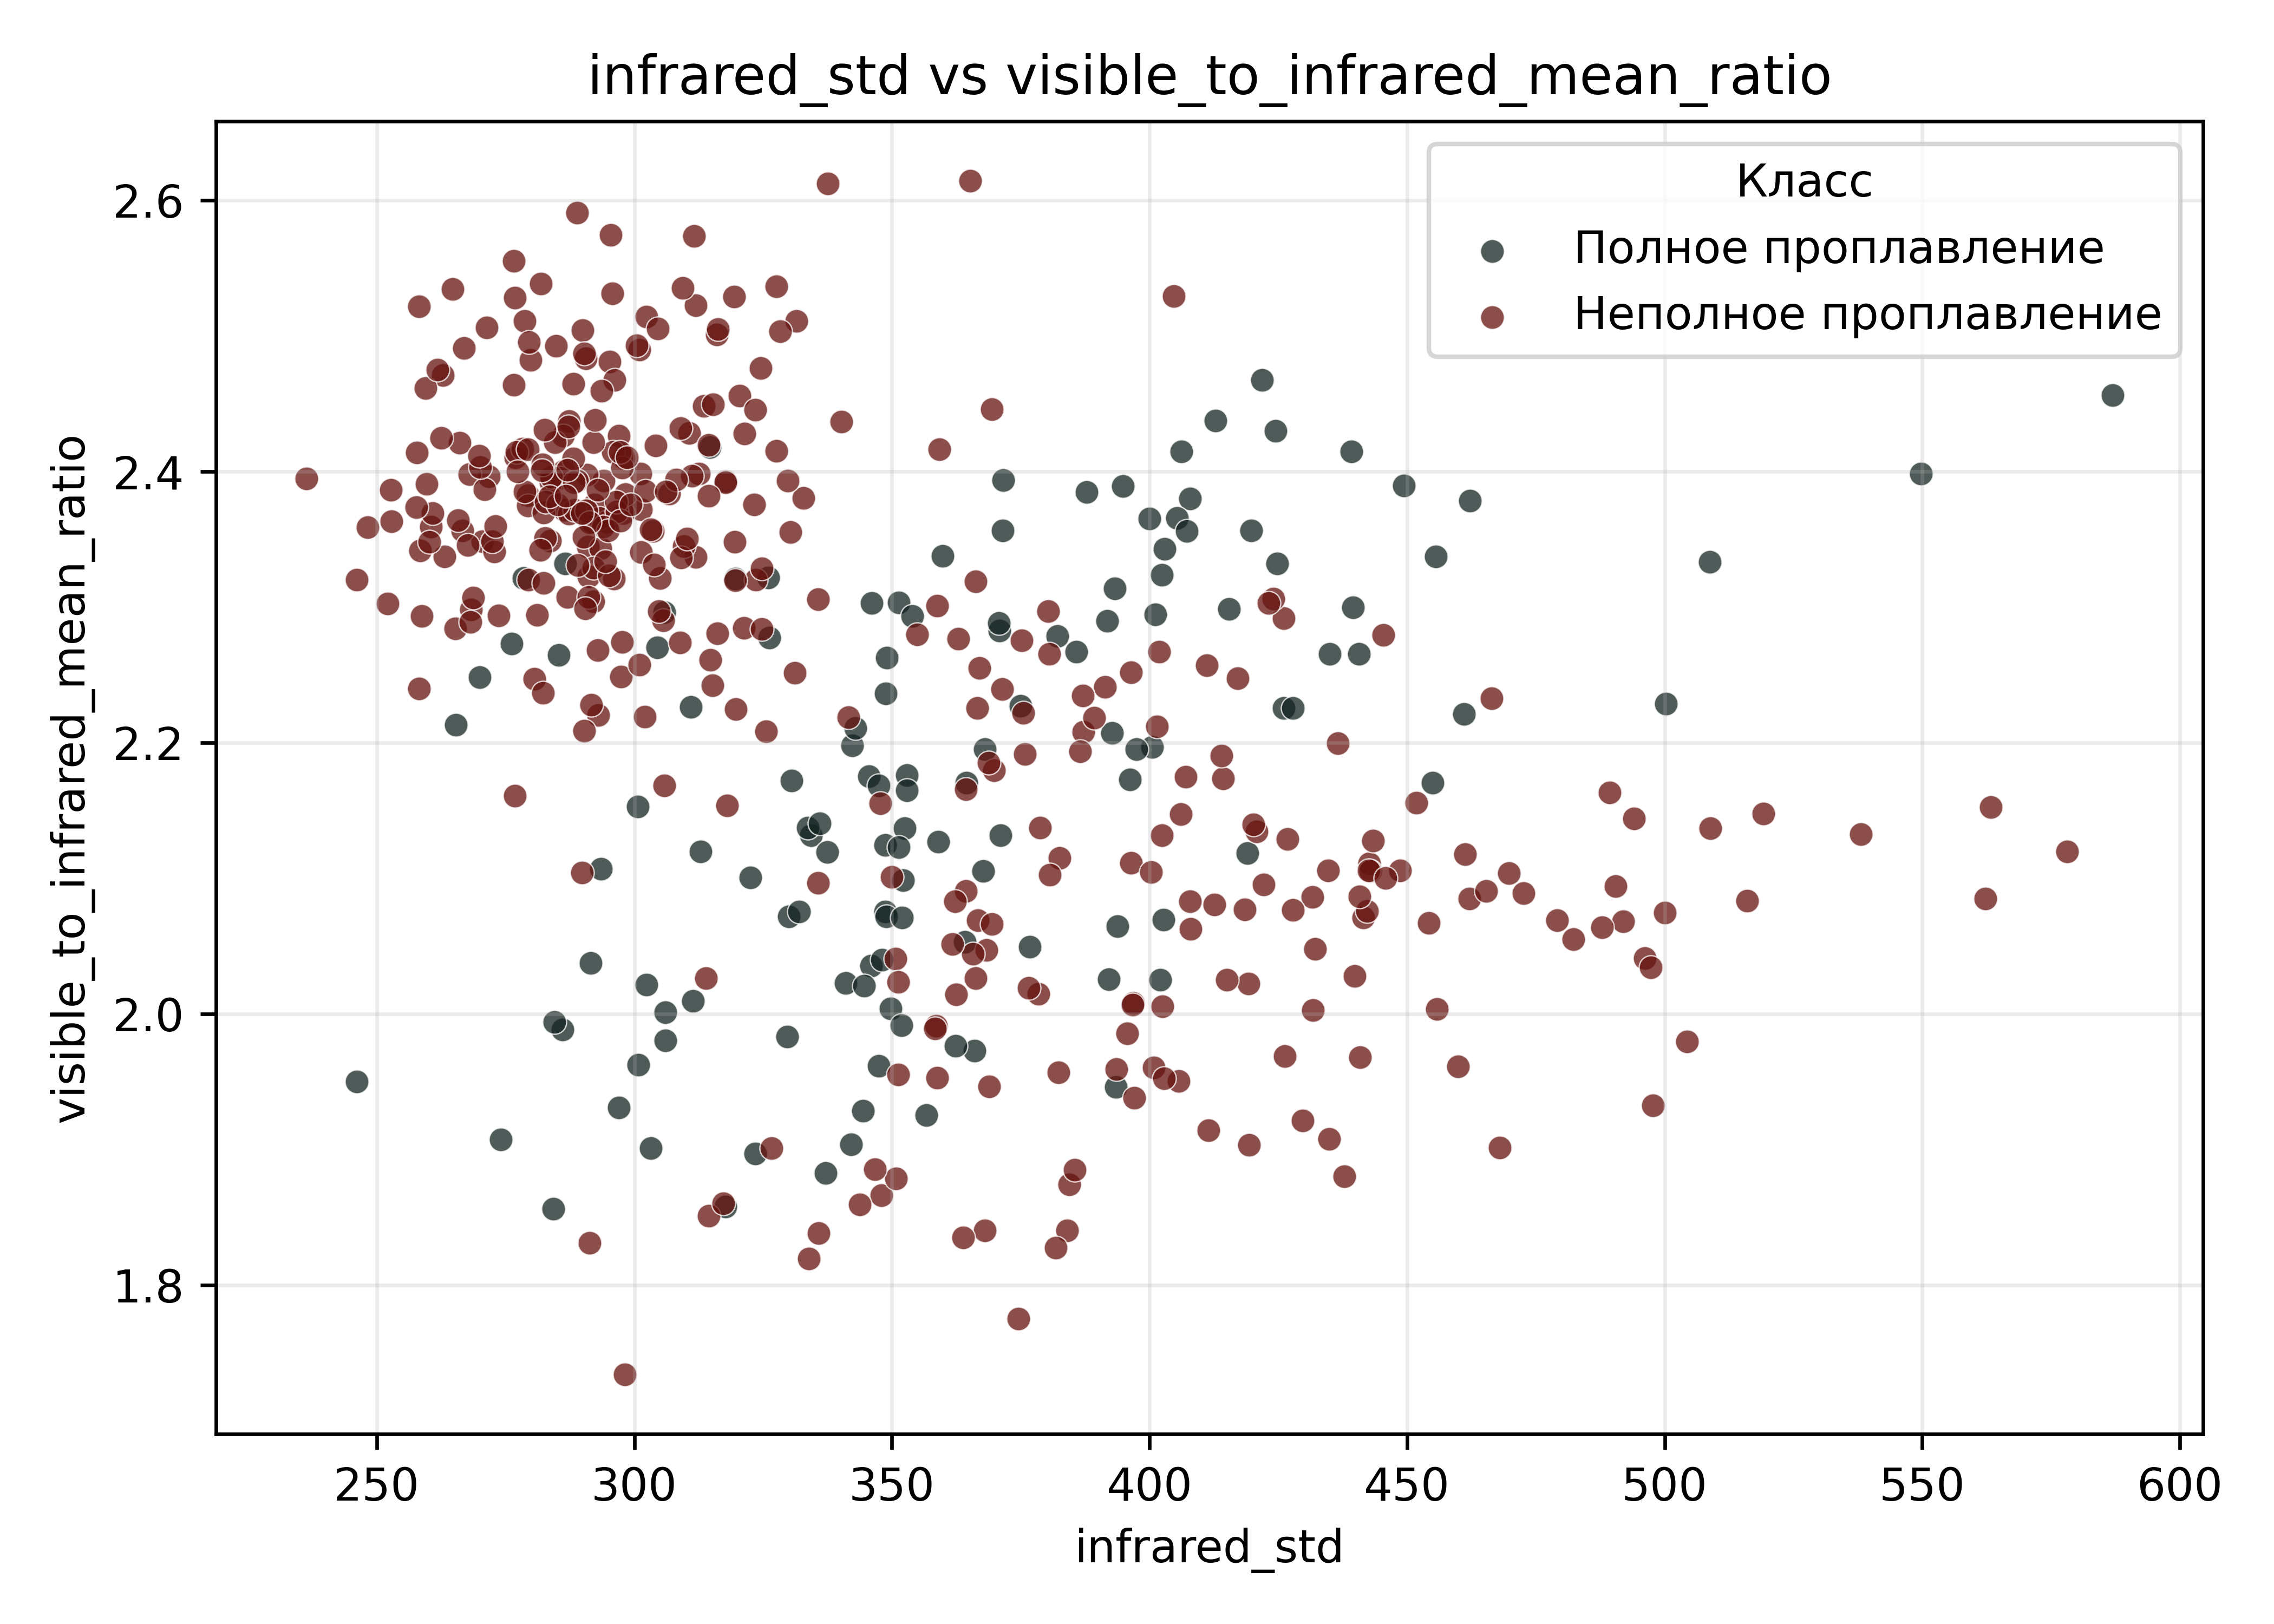
\includegraphics[width=0.78\textwidth]{figures/scatter_infrared_std_vs_visible_to_infrared_mean_ratio.png}
    \caption{Диаграмма рассеяния оконных временных признаков: стандартное отклонение инфракрасного канала и отношение среднего значения видимого канала к среднему значению инфракрасного канала}
    \label{fig:defect_scatter_2}
\end{figure}

Из представленных диаграмм видно, что окна, соответствующие отсутствию непровара и наличию непровара, частично разделяются в пространстве частотных признаков. Наиболее заметно это проявляется в областях, связанных с высокочастотной составляющей сигнала и положением спектрального центроида. При этом полного разделения классов не наблюдается: часть окон с разным состоянием качества располагается в близких областях признакового пространства. Это согласуется с нестационарным характером процесса лазерной сварки и малым числом независимых экспериментальных проходов. Тем не менее наличие частичной разделимости показывает, что частотные признаки видимого и инфракрасного каналов содержат информацию, связанную с формированием непровара.


\section{Качественная оценка непровара без канала отражённого излучения}

Основная качественная постановка задачи состояла в определении наличия непровара по оконным признакам. Бинарная метка качества задавалась по величине \(h_i\):
\[
    y =
    \begin{cases}
        0, & h_i = 0, \\
        1, & h_i > 0.
    \end{cases}
\]
Здесь \(y=0\) соответствует отсутствию непровара, а \(y=1\) --- наличию непровара.

В качестве основного варианта рассматривалась классификация без использования канала отражённого лазерного излучения. Это связано с тем, что канал отражённого излучения в данном наборе данных тесно связан с мощностью лазерного излучения, что ведет к потенциальному переобучению модели. Поэтому сначала было проверено, возможно ли определить наличие непровара по сигналам видимого и инфракрасного каналов.

Для классификации использовались LDA, Logistic Regression, SVM-linear, SVM-RBF, k-NN, Random Forest и Gradient Boosting. Качество моделей оценивалось с использованием оконной кросс-валидации. Отдельное окно рассматривается как локальный фрагмент процесса, по которому требуется принять решение о наличии или отсутствии непровара.

Результаты сравнения классификаторов без использования канала отражённого излучения приведены на рис.~\ref{fig:defect_classifier_comparison_no_reflected}. На диаграмме высота столбца соответствует среднему значению метрики качества, вертикальные отрезки показывают разброс результата по отдельным разбиениям кросс-валидации, а точки соответствуют значениям метрики на отдельных разбиениях.

\begin{figure}[H]
    \centering
    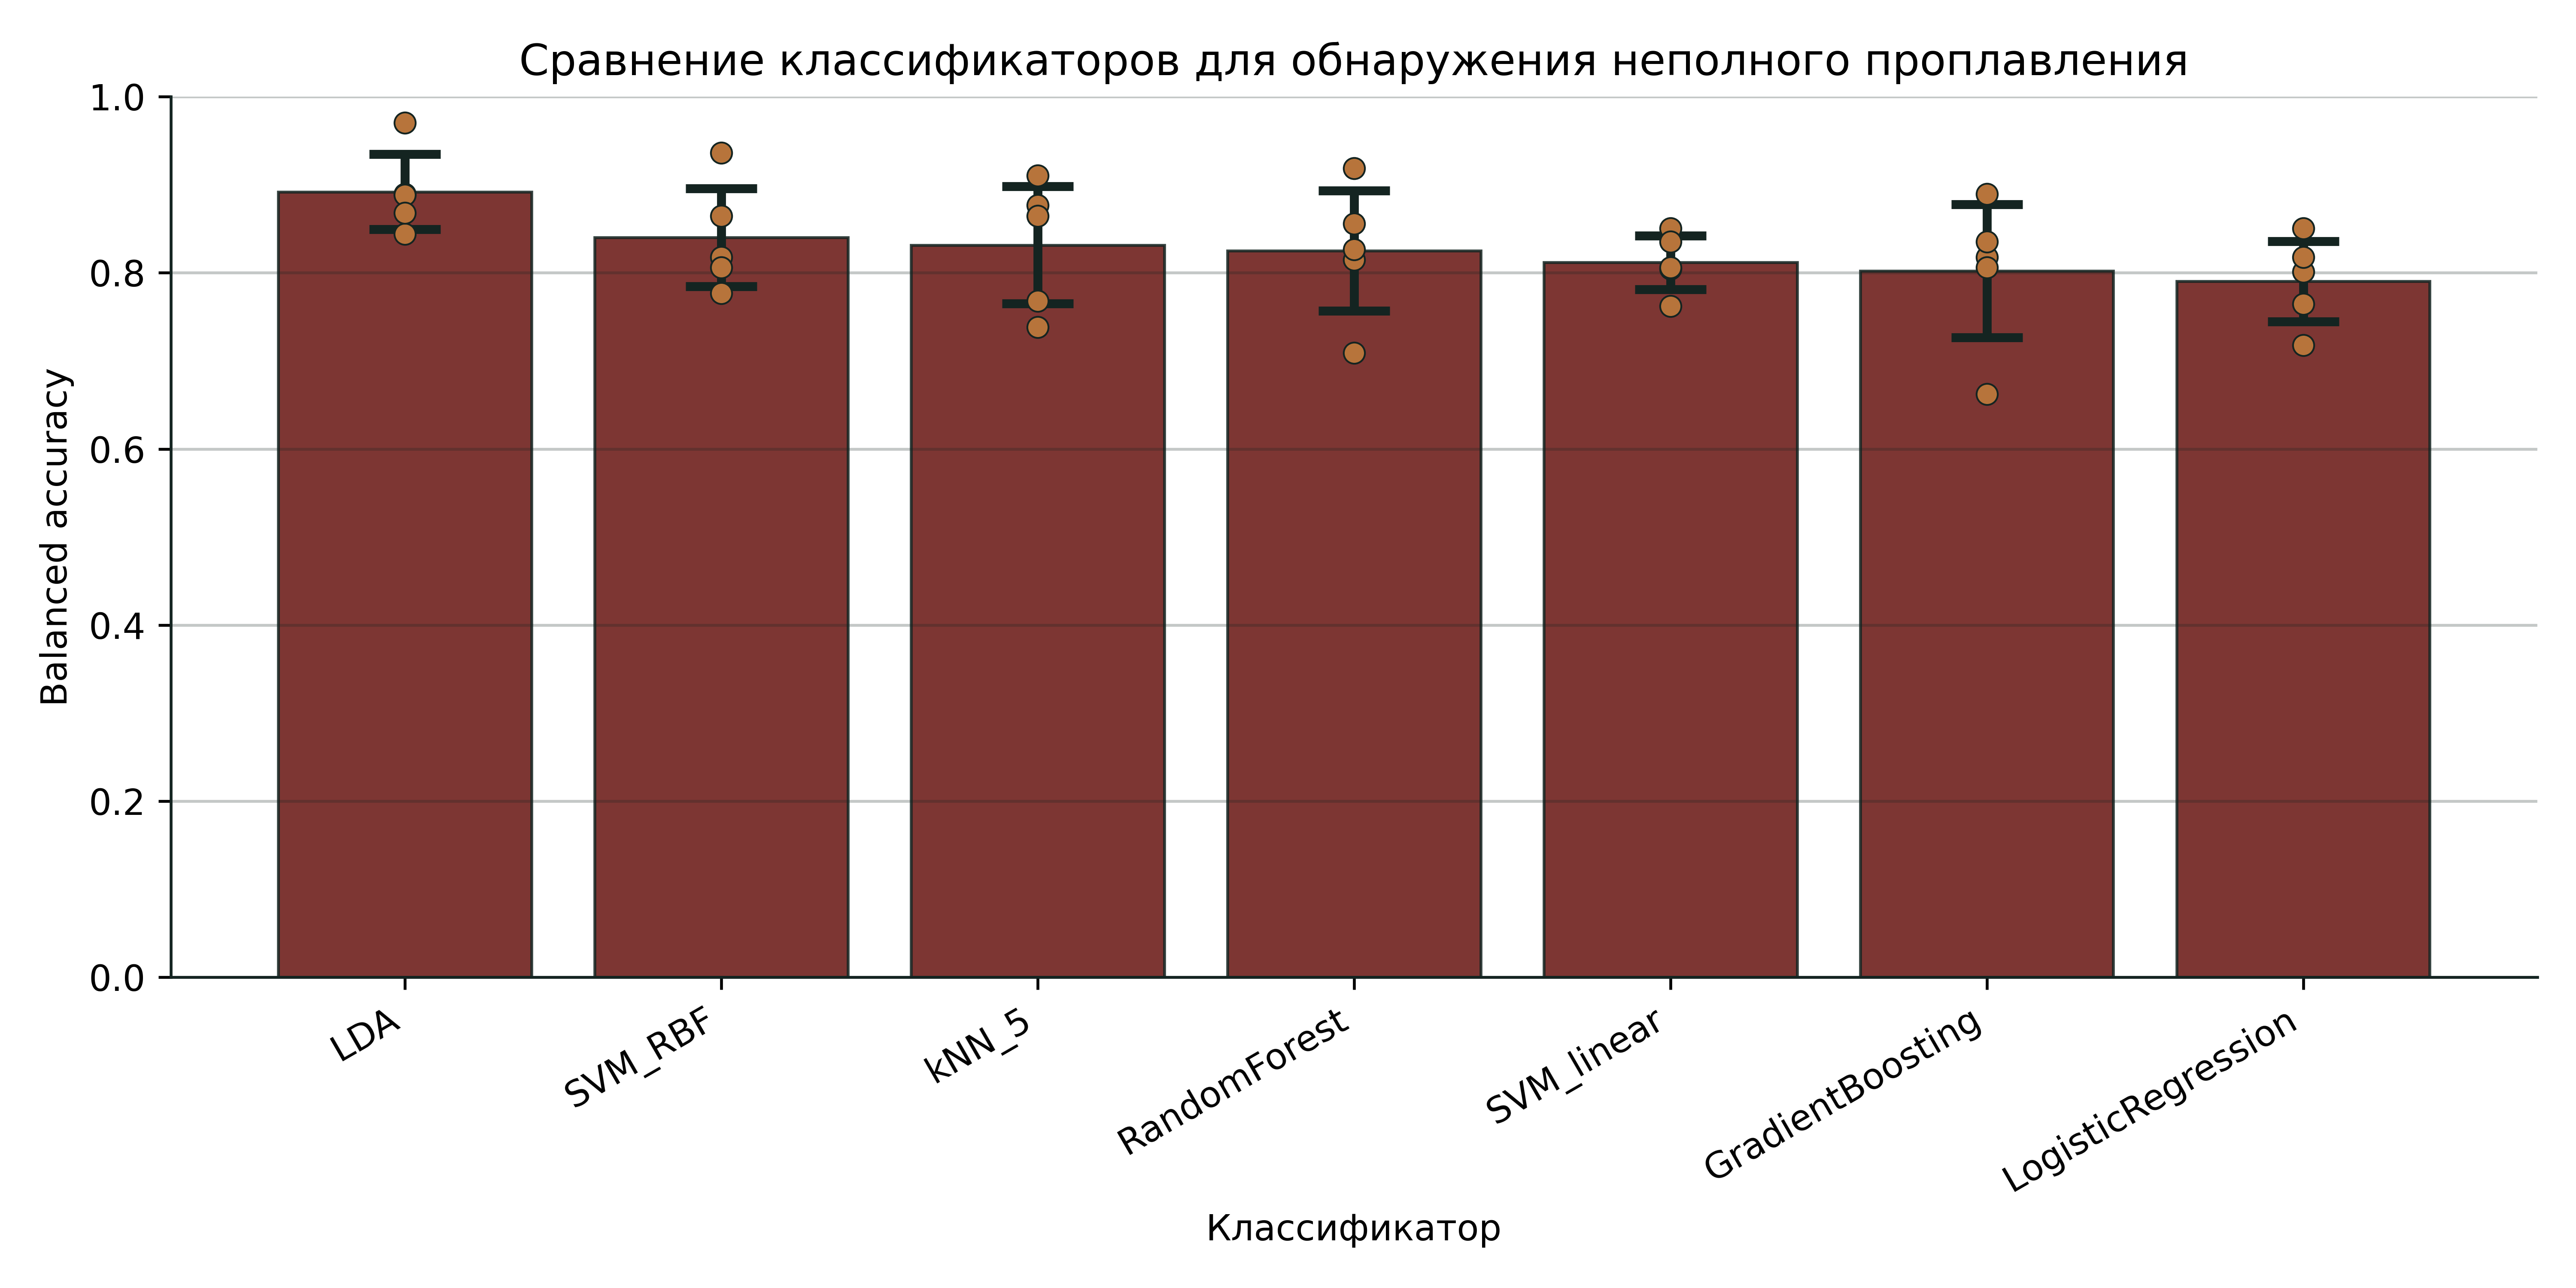
\includegraphics[width=0.86\textwidth]{figures/defect_classifier_comparison.png}
    \caption{Сравнение классификаторов при обнаружении непровара без использования канала отражённого излучения}
    \label{fig:defect_classifier_comparison_no_reflected}
\end{figure}

Для более детального анализа ошибок была построена нормированная матрица ошибок для модели LDA. В матрице строки соответствуют фактическим классам, а столбцы --- классам, предсказанным моделью. Элементы матрицы показывают долю окон данного фактического класса, отнесённых классификатором к каждому из классов.

\begin{figure}[H]
    \centering
    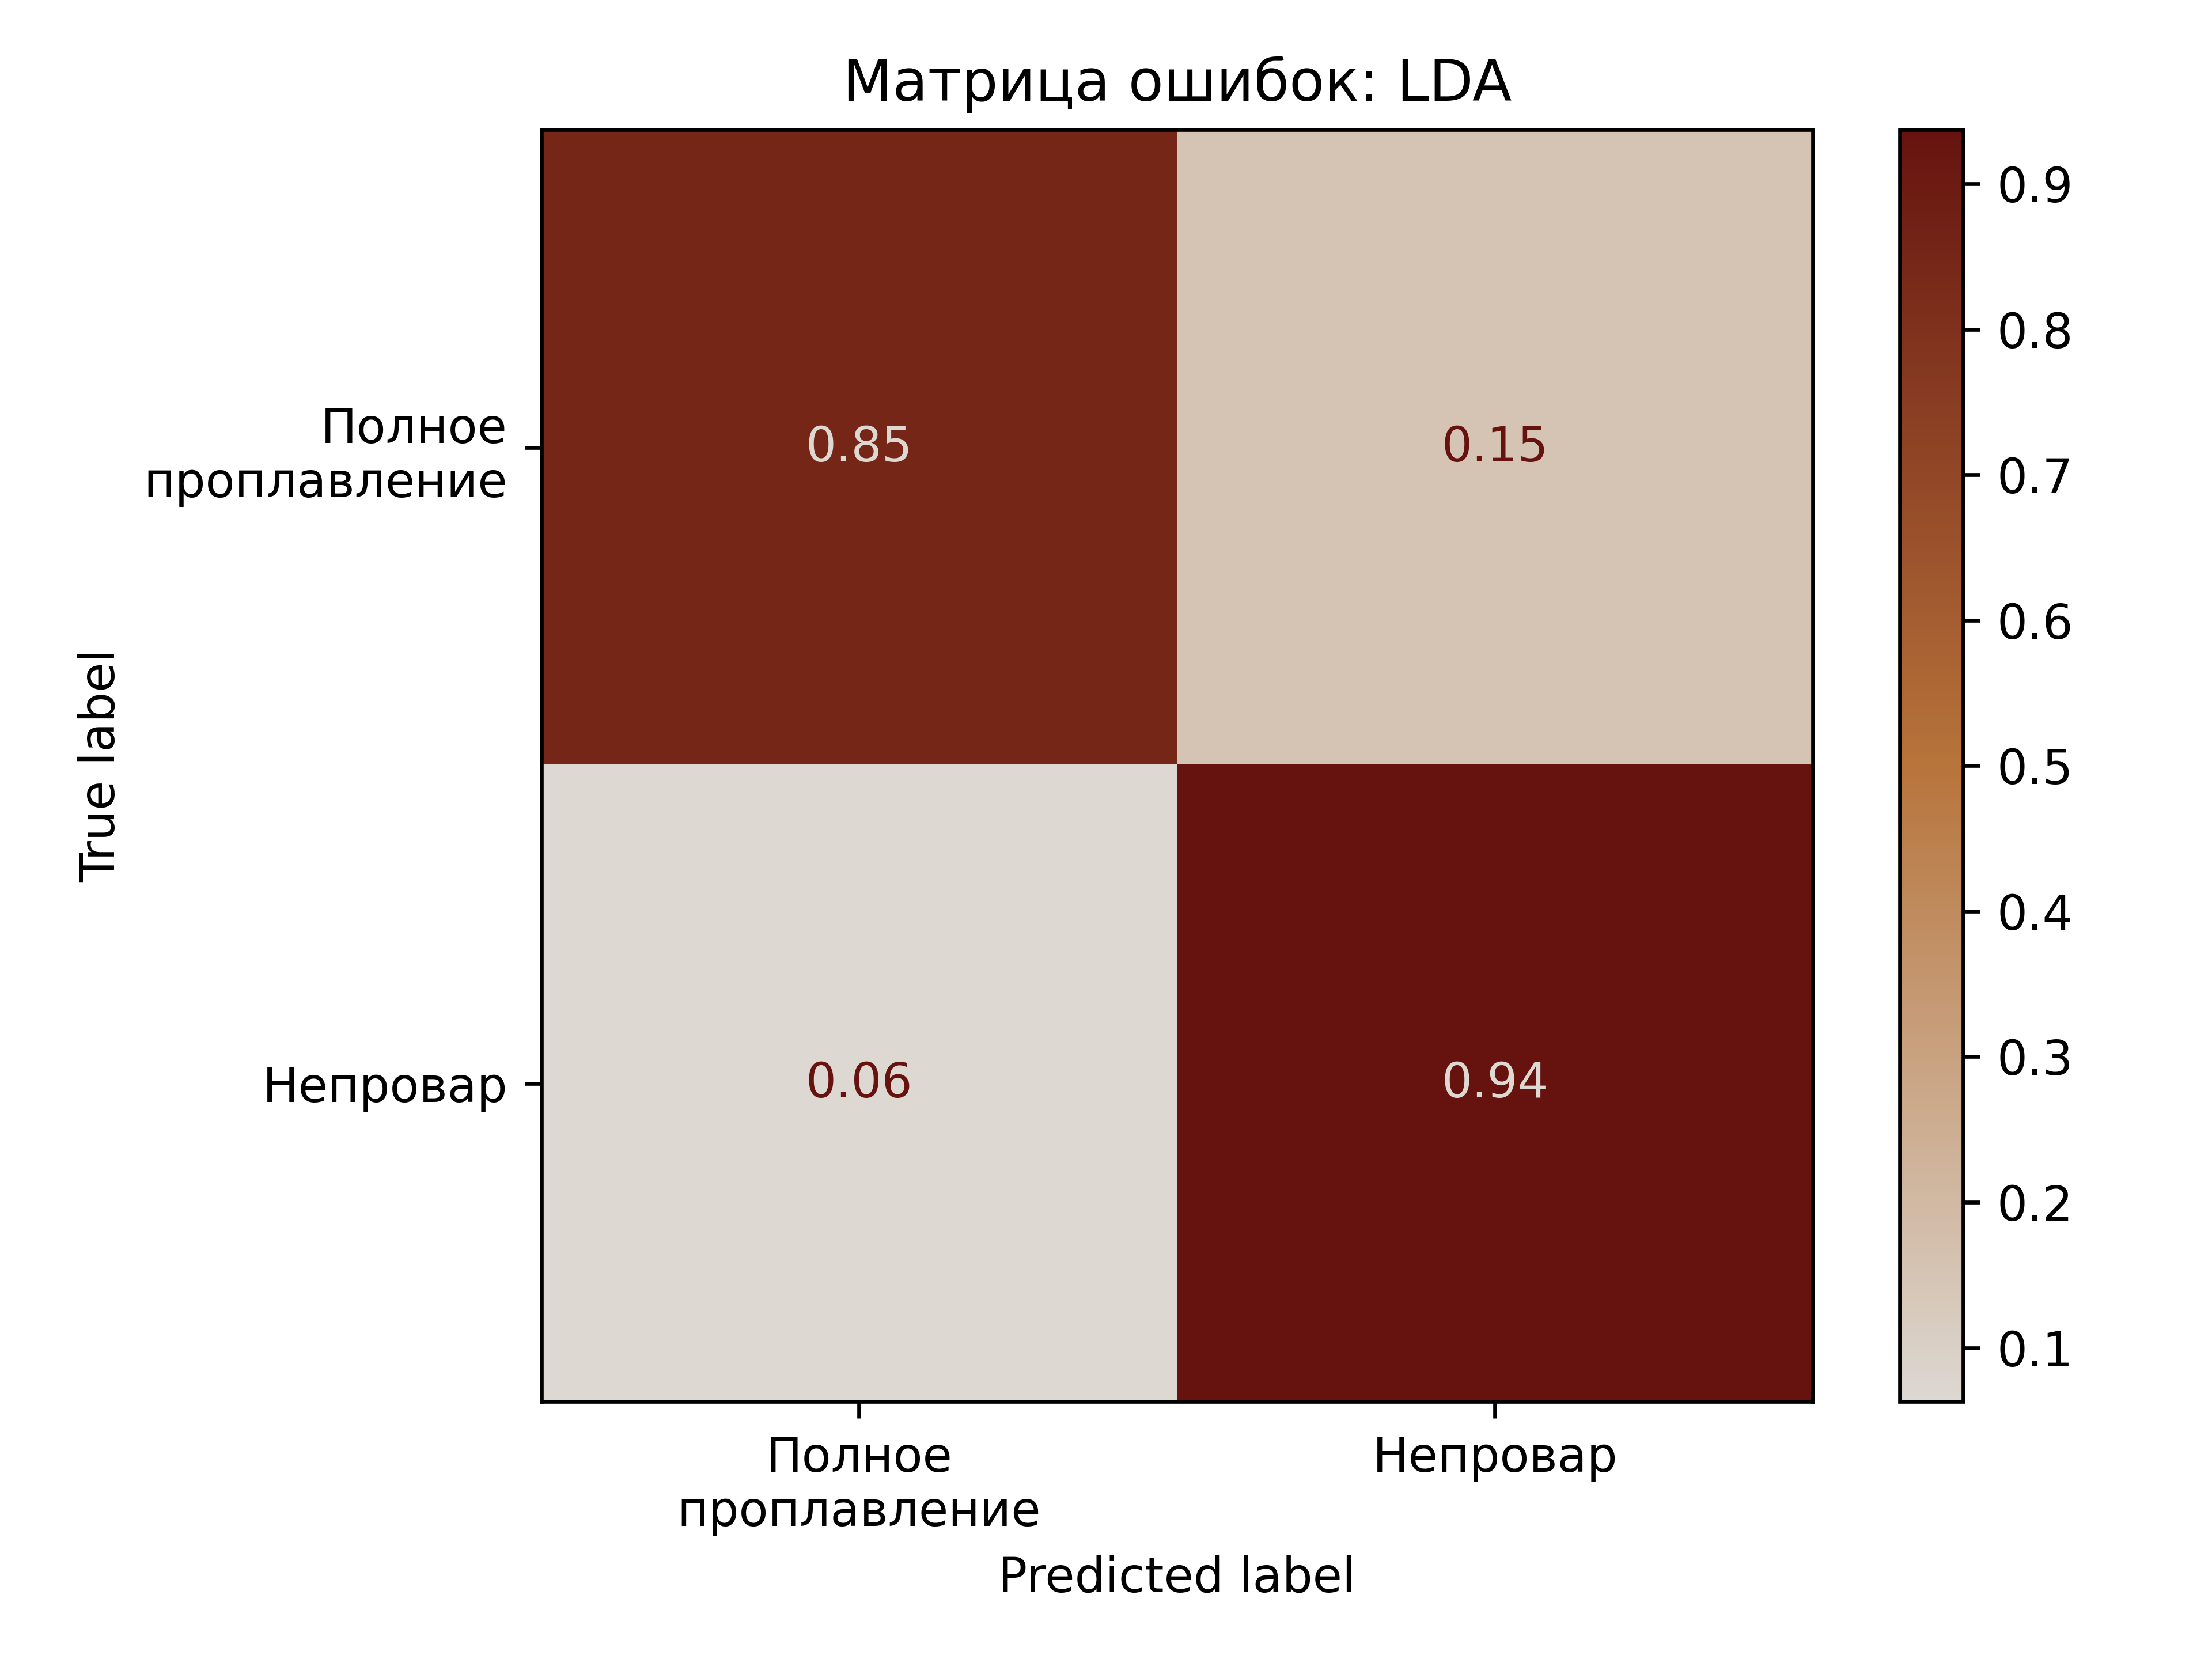
\includegraphics[width=0.65\textwidth]{figures/defect_confusion_matrix.png}
    \caption{Нормированная матрица ошибок для бинарной классификации непровара без использования канала отражённого излучения}
    \label{fig:defect_confusion_matrix_lda_no_reflected}
\end{figure}

Согласно полученной матрице ошибок, отсутствие непровара корректно определялось с вероятностью 85~\%, а наличие непровара 94~\%. Таким образом, качественная оценка непровара оказалась возможной даже без использования канала отражённого излучения. Этот результат показывает, что признаки видимого и инфракрасного каналов содержат информацию, связанную с качеством формирования сварного соединения.

\section{Роль канала отражённого излучения}

Канал отражённого лазерного излучения был рассмотрен отдельно. Его особенность состоит в том, что уровень отражённого сигнала заметно связан с мощностью лазерного излучения. В рассматриваемой серии экспериментов величина \(h_i\) также изменялась совместно с мощностью: при увеличении мощности величина непровара уменьшалась. Поэтому при включении канала отражённого излучения модель может использовать его как косвенный признак режима мощности.

С инженерной точки зрения это не делает канал отраженного бесполезным: он действительно входит в состав регистрируемого оптического отклика процесса. Однако для интерпретации результатов важно учитывать структуру исходного набора данных. При малом числе экспериментов и дискретном наборе мощностей чрезмерно высокая информативность отражённого канала может приводить к переобучению модели --- завышенной оценке качества на обучающей выборке.

Для проверки влияния отражённого канала была выполнена классификация с использованием всех трёх каналов фотодиодной системы. Результаты сравнения классификаторов приведены на рис.~\ref{fig:defect_classifier_comparison_with_reflected}.

\begin{figure}[H]
    \centering
    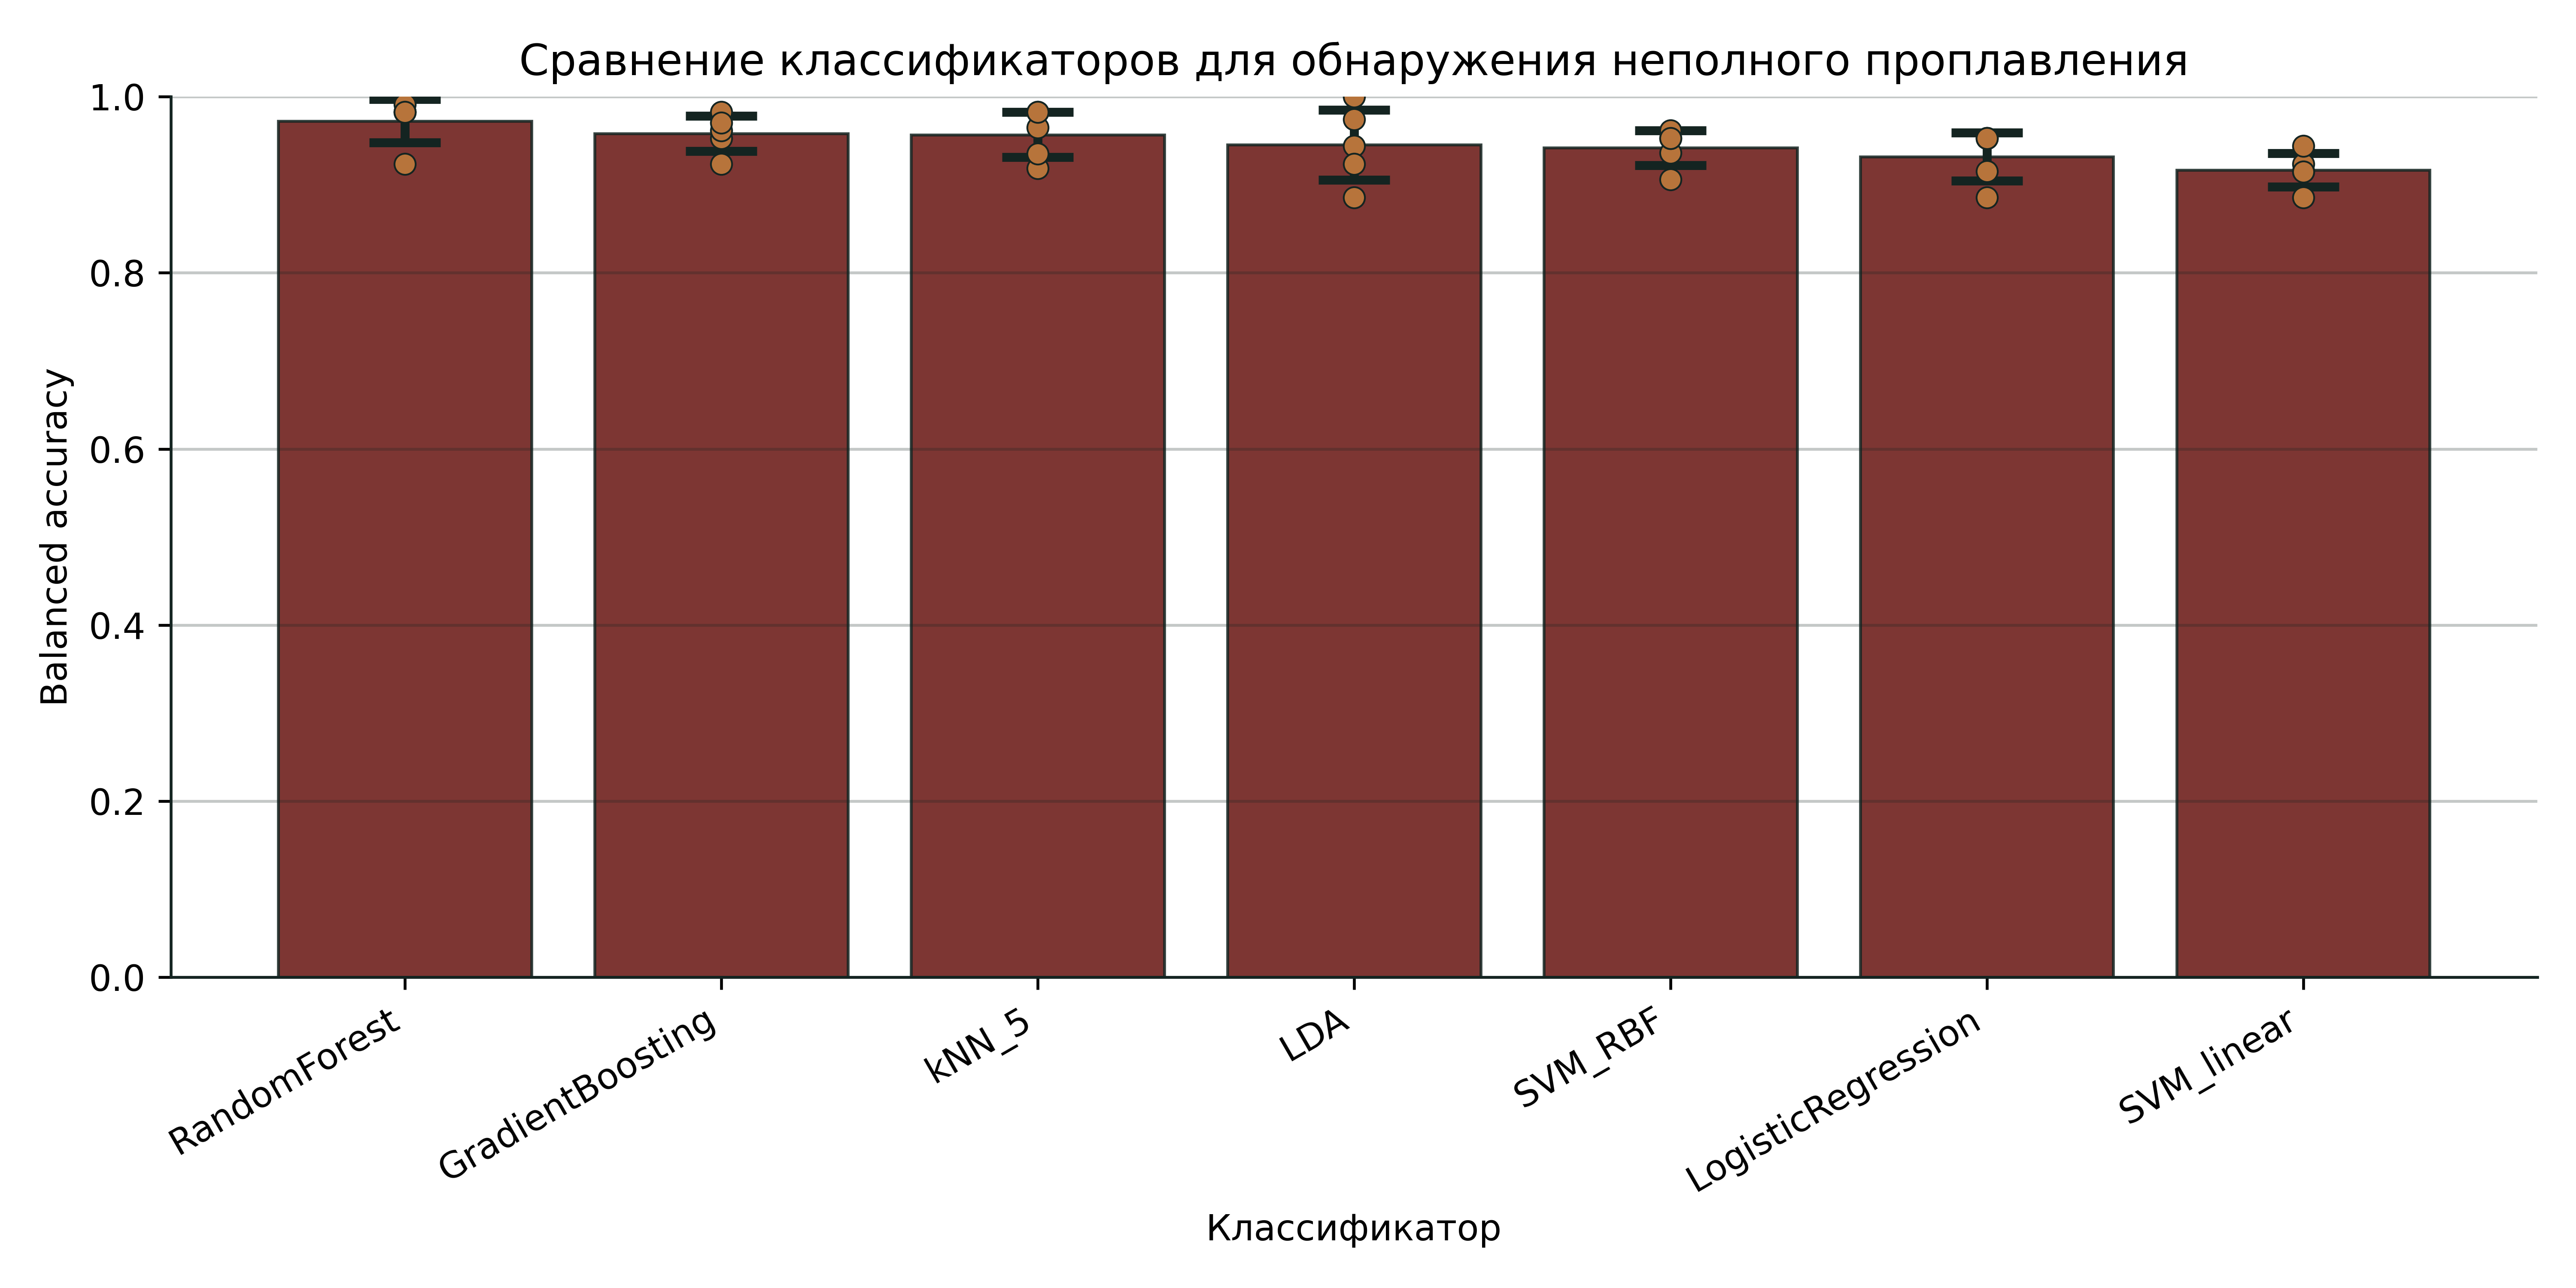
\includegraphics[width=0.86\textwidth]{figures/defect_classifier_comparison_reflected.png}
    \caption{Сравнение классификаторов при обнаружении непровара с использованием всех каналов фотодиодной системы}
    \label{fig:defect_classifier_comparison_with_reflected}
\end{figure}

Добавление канала отражённого излучения значительно повышало качество классификации. Однако такой результат следует рассматривать с учётом того, что в данной серии экспериментов отражённый канал связан с мощностью, а мощность, в свою очередь, связана с величиной \(h_i\). Поэтому основным выводом является возможность качественного обнаружения непровара без использования канала отражённого излучения.

\section{Количественная оценка величины непровара}

После проверки качественной постановки была рассмотрена возможность количественной оценки непровара. В этом случае задача формулировалась как регрессия: по оконным признакам фотодиодных сигналов требовалось оценить численное значение \(h_i\). В качестве метрик использовались средняя абсолютная ошибка MAE, среднеквадратичная ошибка RMSE и коэффициент детерминации \(R^2\). Основное внимание уделялось MAE, поскольку эта метрика выражается в миллиметрах и непосредственно показывает среднюю ошибку оценки \(h_i\).

На первом этапе регрессия была выполнена без использования канала отражённого излучения. Такой вариант позволяет проверить, насколько устойчиво величина непровара может быть оценена только по сигналам видимого и инфракрасного каналов. Для сравнения были использованы несколько регрессионных моделей: Linear Regression, Ridge, Lasso, SVR, k-NN, Random Forest и Gradient Boosting.

Результаты сравнения регрессионных моделей без использования канала отражённого излучения приведены на рис.~\ref{fig:hi_regression_comparison_no_reflected}. На диаграмме высота столбца соответствует среднему значению MAE по разбиениям кросс-валидации. Вертикальные отрезки показывают стандартное отклонение MAE, а отдельные точки соответствуют значениям ошибки на конкретных разбиениях. Поскольку MAE является ошибкой прогноза, меньшие значения данной метрики соответствуют более точной модели.

\begin{figure}[H]
    \centering
    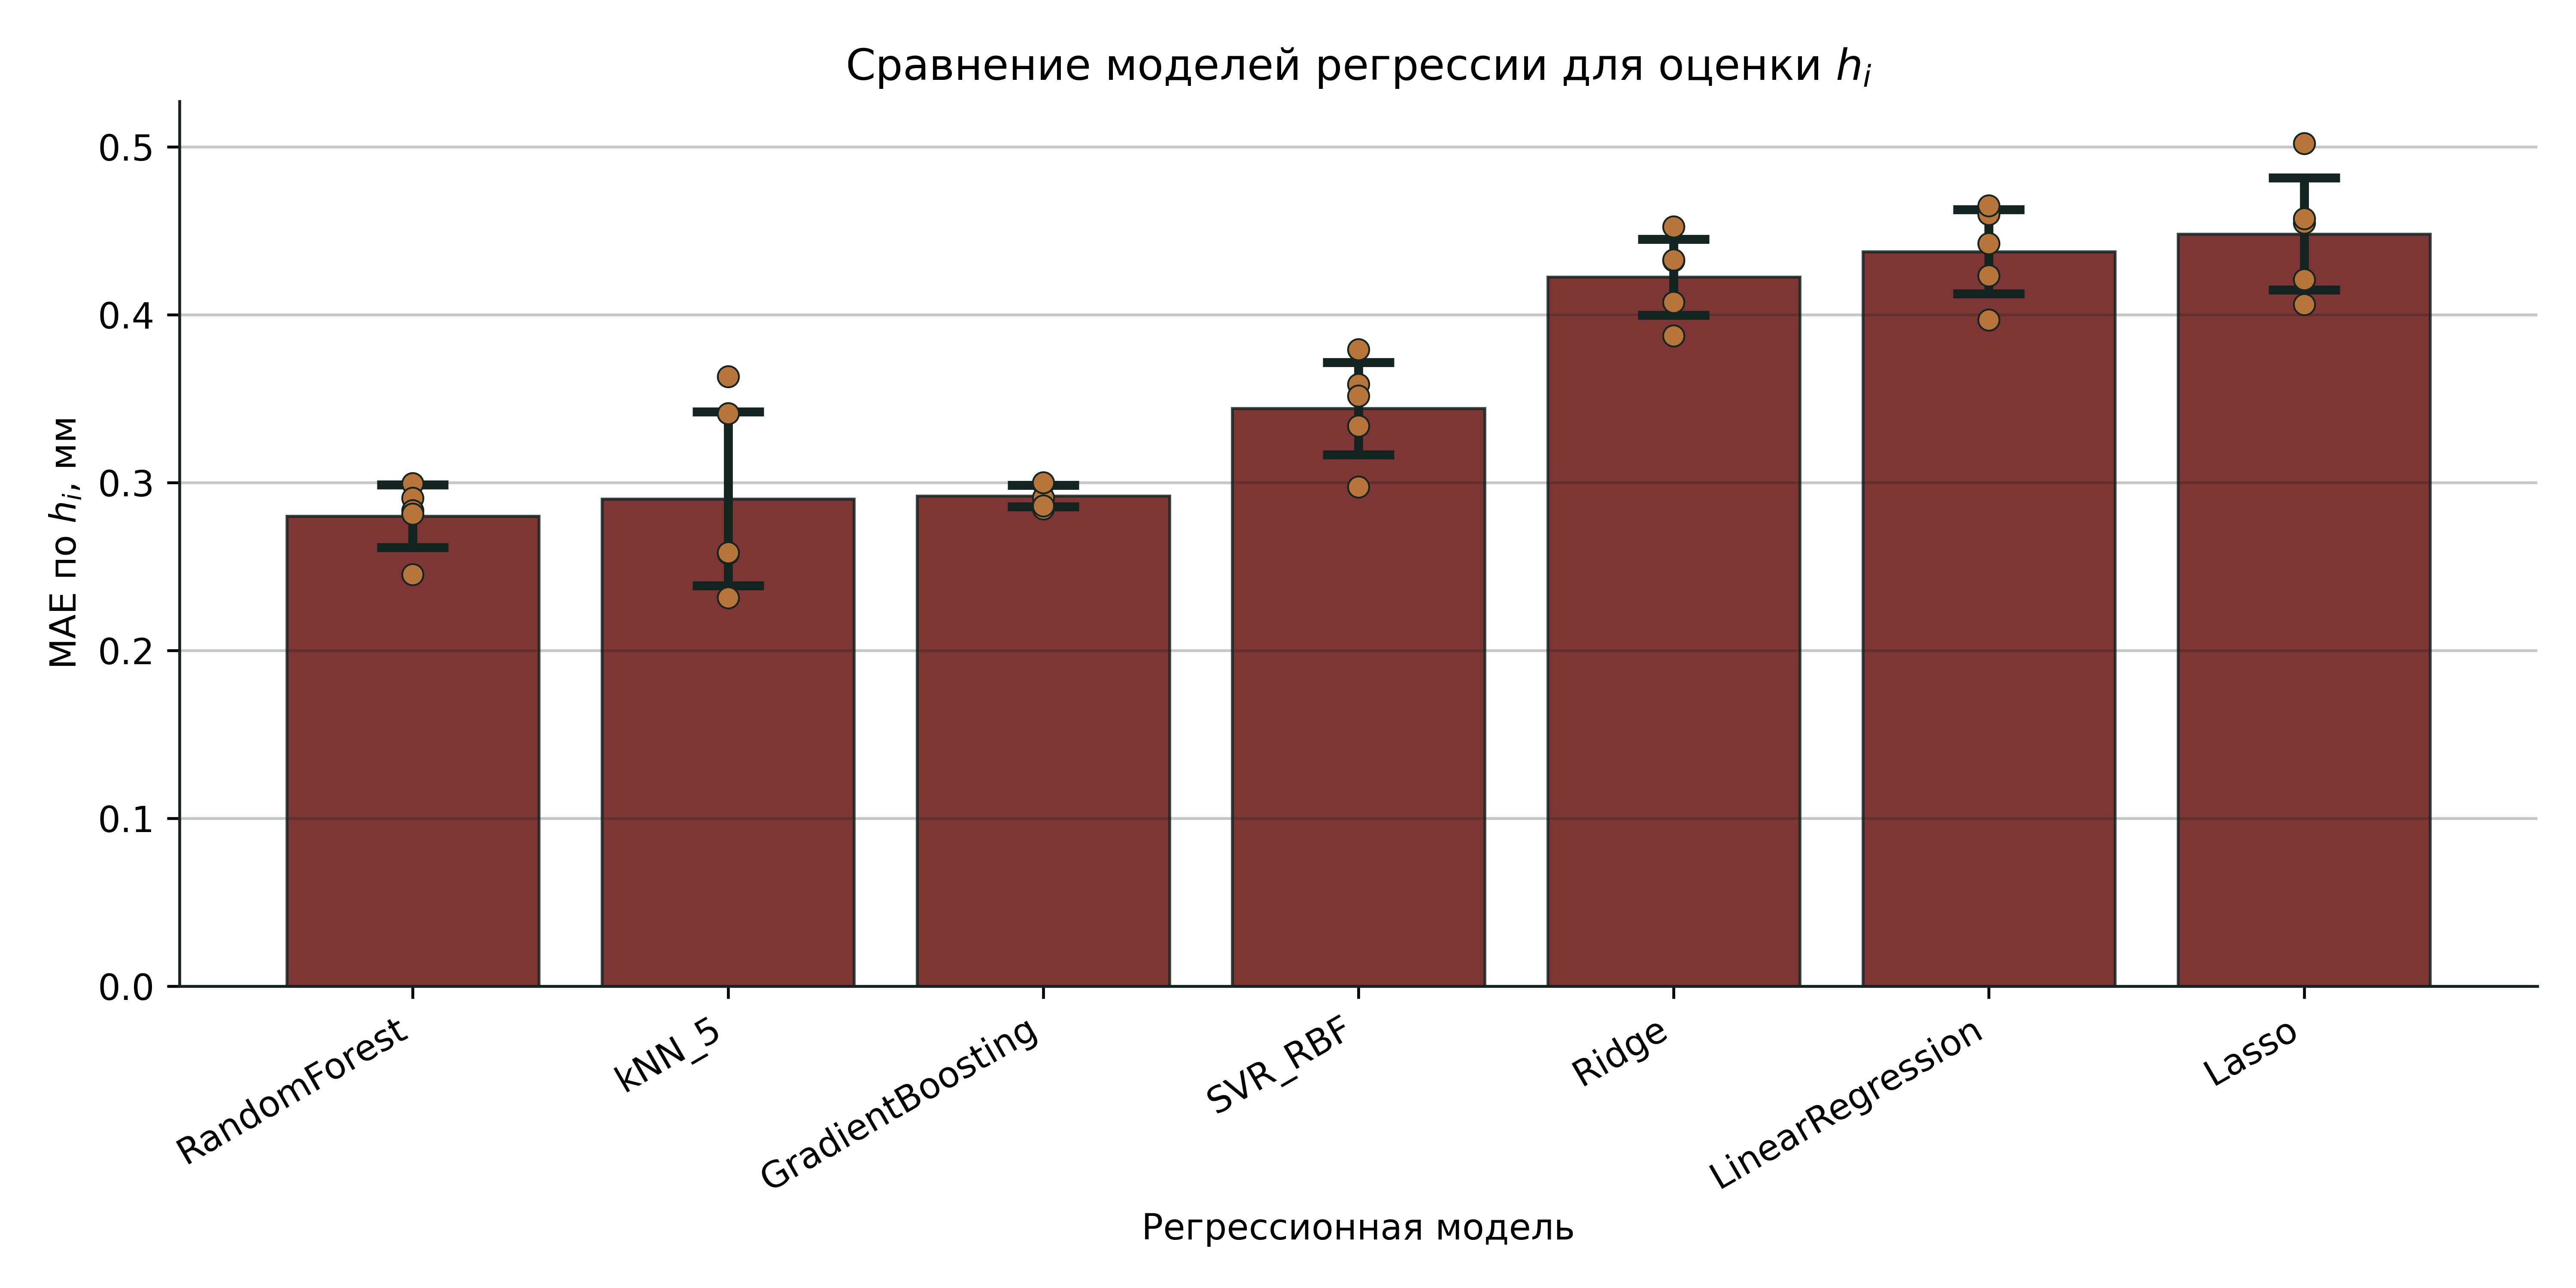
\includegraphics[width=0.86\textwidth]{figures/hi_regression_comparison_no_reflected.png}
    \caption{Сравнение регрессионных моделей при оценке \(h_i\) без использования канала отражённого излучения}
    \label{fig:hi_regression_comparison_no_reflected}
\end{figure}

В варианте без канала отражённого излучения наилучший результат был получен с использованием модели Random Forest. На рис.~\ref{fig:hi_regression_no_reflected} показано распределение предсказанных значений \(h_i\) по окнам для различных фактических значений. Диаграммы типа ``ящик с усами'' отражают разброс оконных предсказаний, а пунктирная линия соответствует идеальному соотношению между фактическим и предсказанным значением.

\begin{figure}[H]
    \centering
    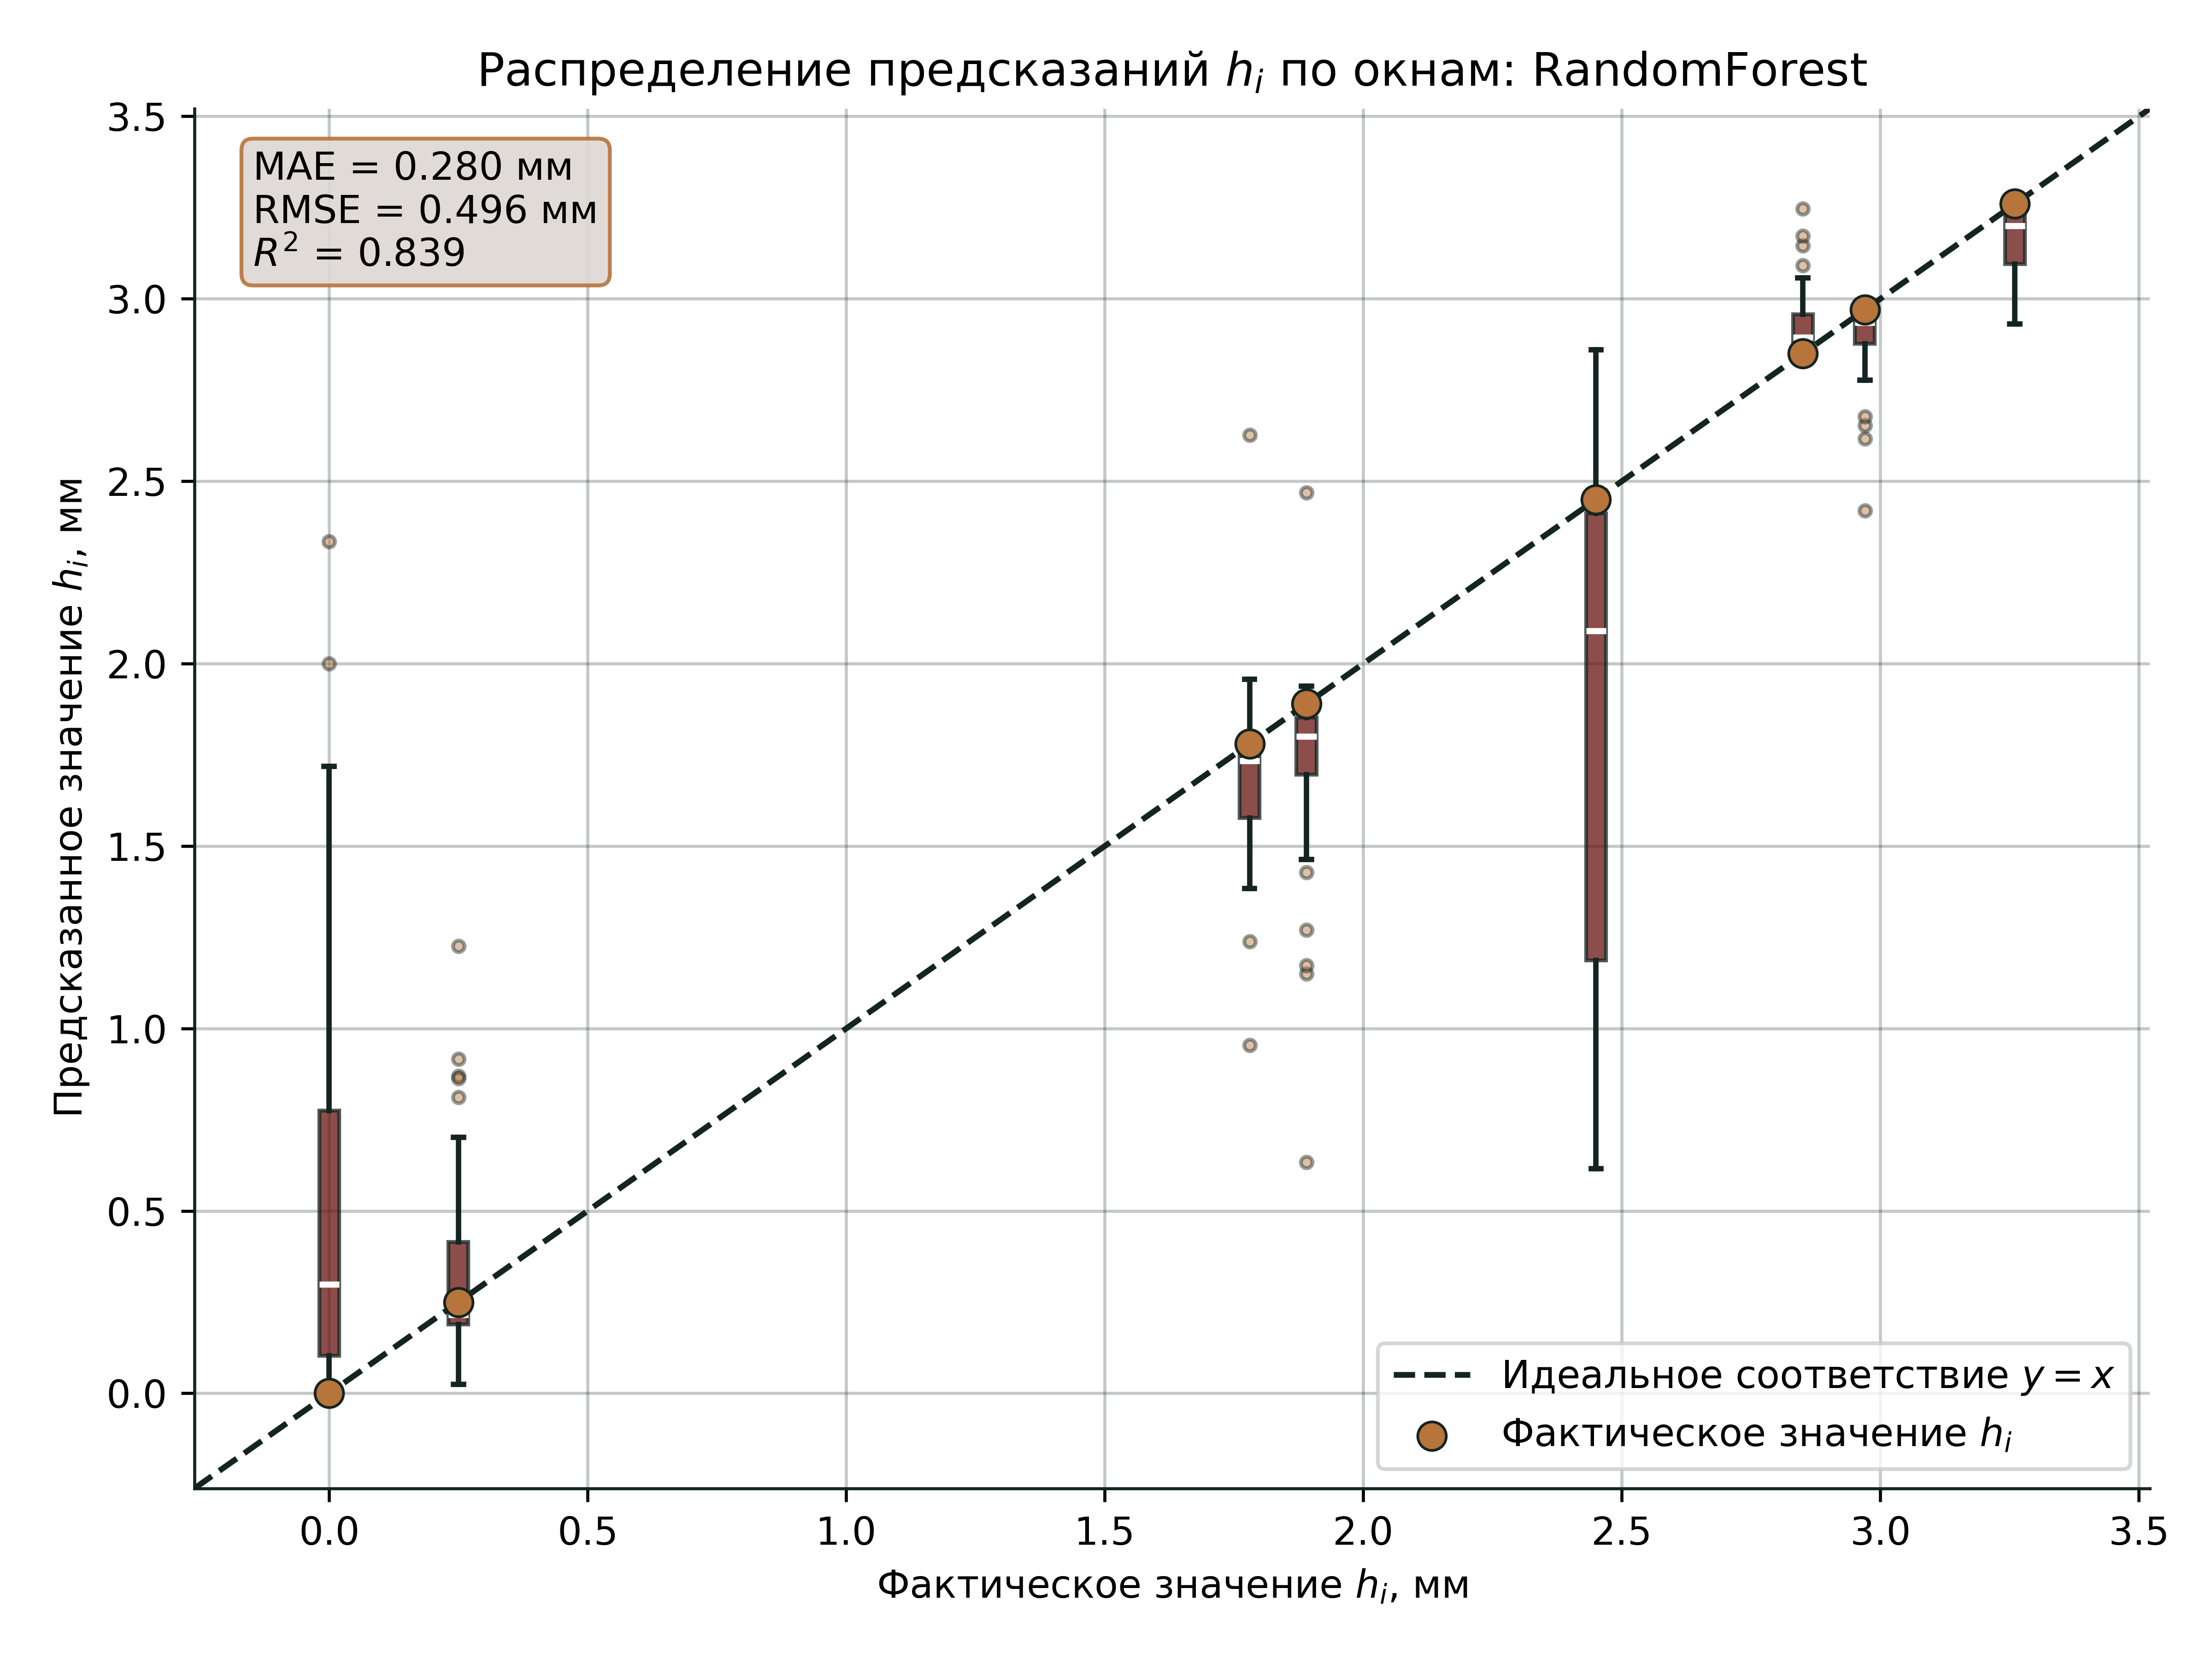
\includegraphics[width=0.78\textwidth]{figures/hi_regression_no_reflected.png}
    \caption{Распределение предсказанных значений \(h_i\) по окнам без использования канала отражённого излучения}
    \label{fig:hi_regression_no_reflected}
\end{figure}

Для варианта без канала отражённого излучения средняя абсолютная ошибка составила 0.28~мм. При этом распределения предсказанных значений имеют заметный разброс, что указывает на недостаточную устойчивость количественной оценки \(h_i\) только по видимому и инфракрасному каналам.

Затем была выполнена регрессия с использованием всех трёх каналов фотодиодной системы. Этот вариант позволяет оценить, насколько изменяется качество количественного прогноза при добавлении канала отражённого лазерного излучения. Результаты сравнения регрессионных моделей для данного случая приведены на рис.~\ref{fig:hi_regression_comparison_with_reflected}.

\begin{figure}[H]
    \centering
    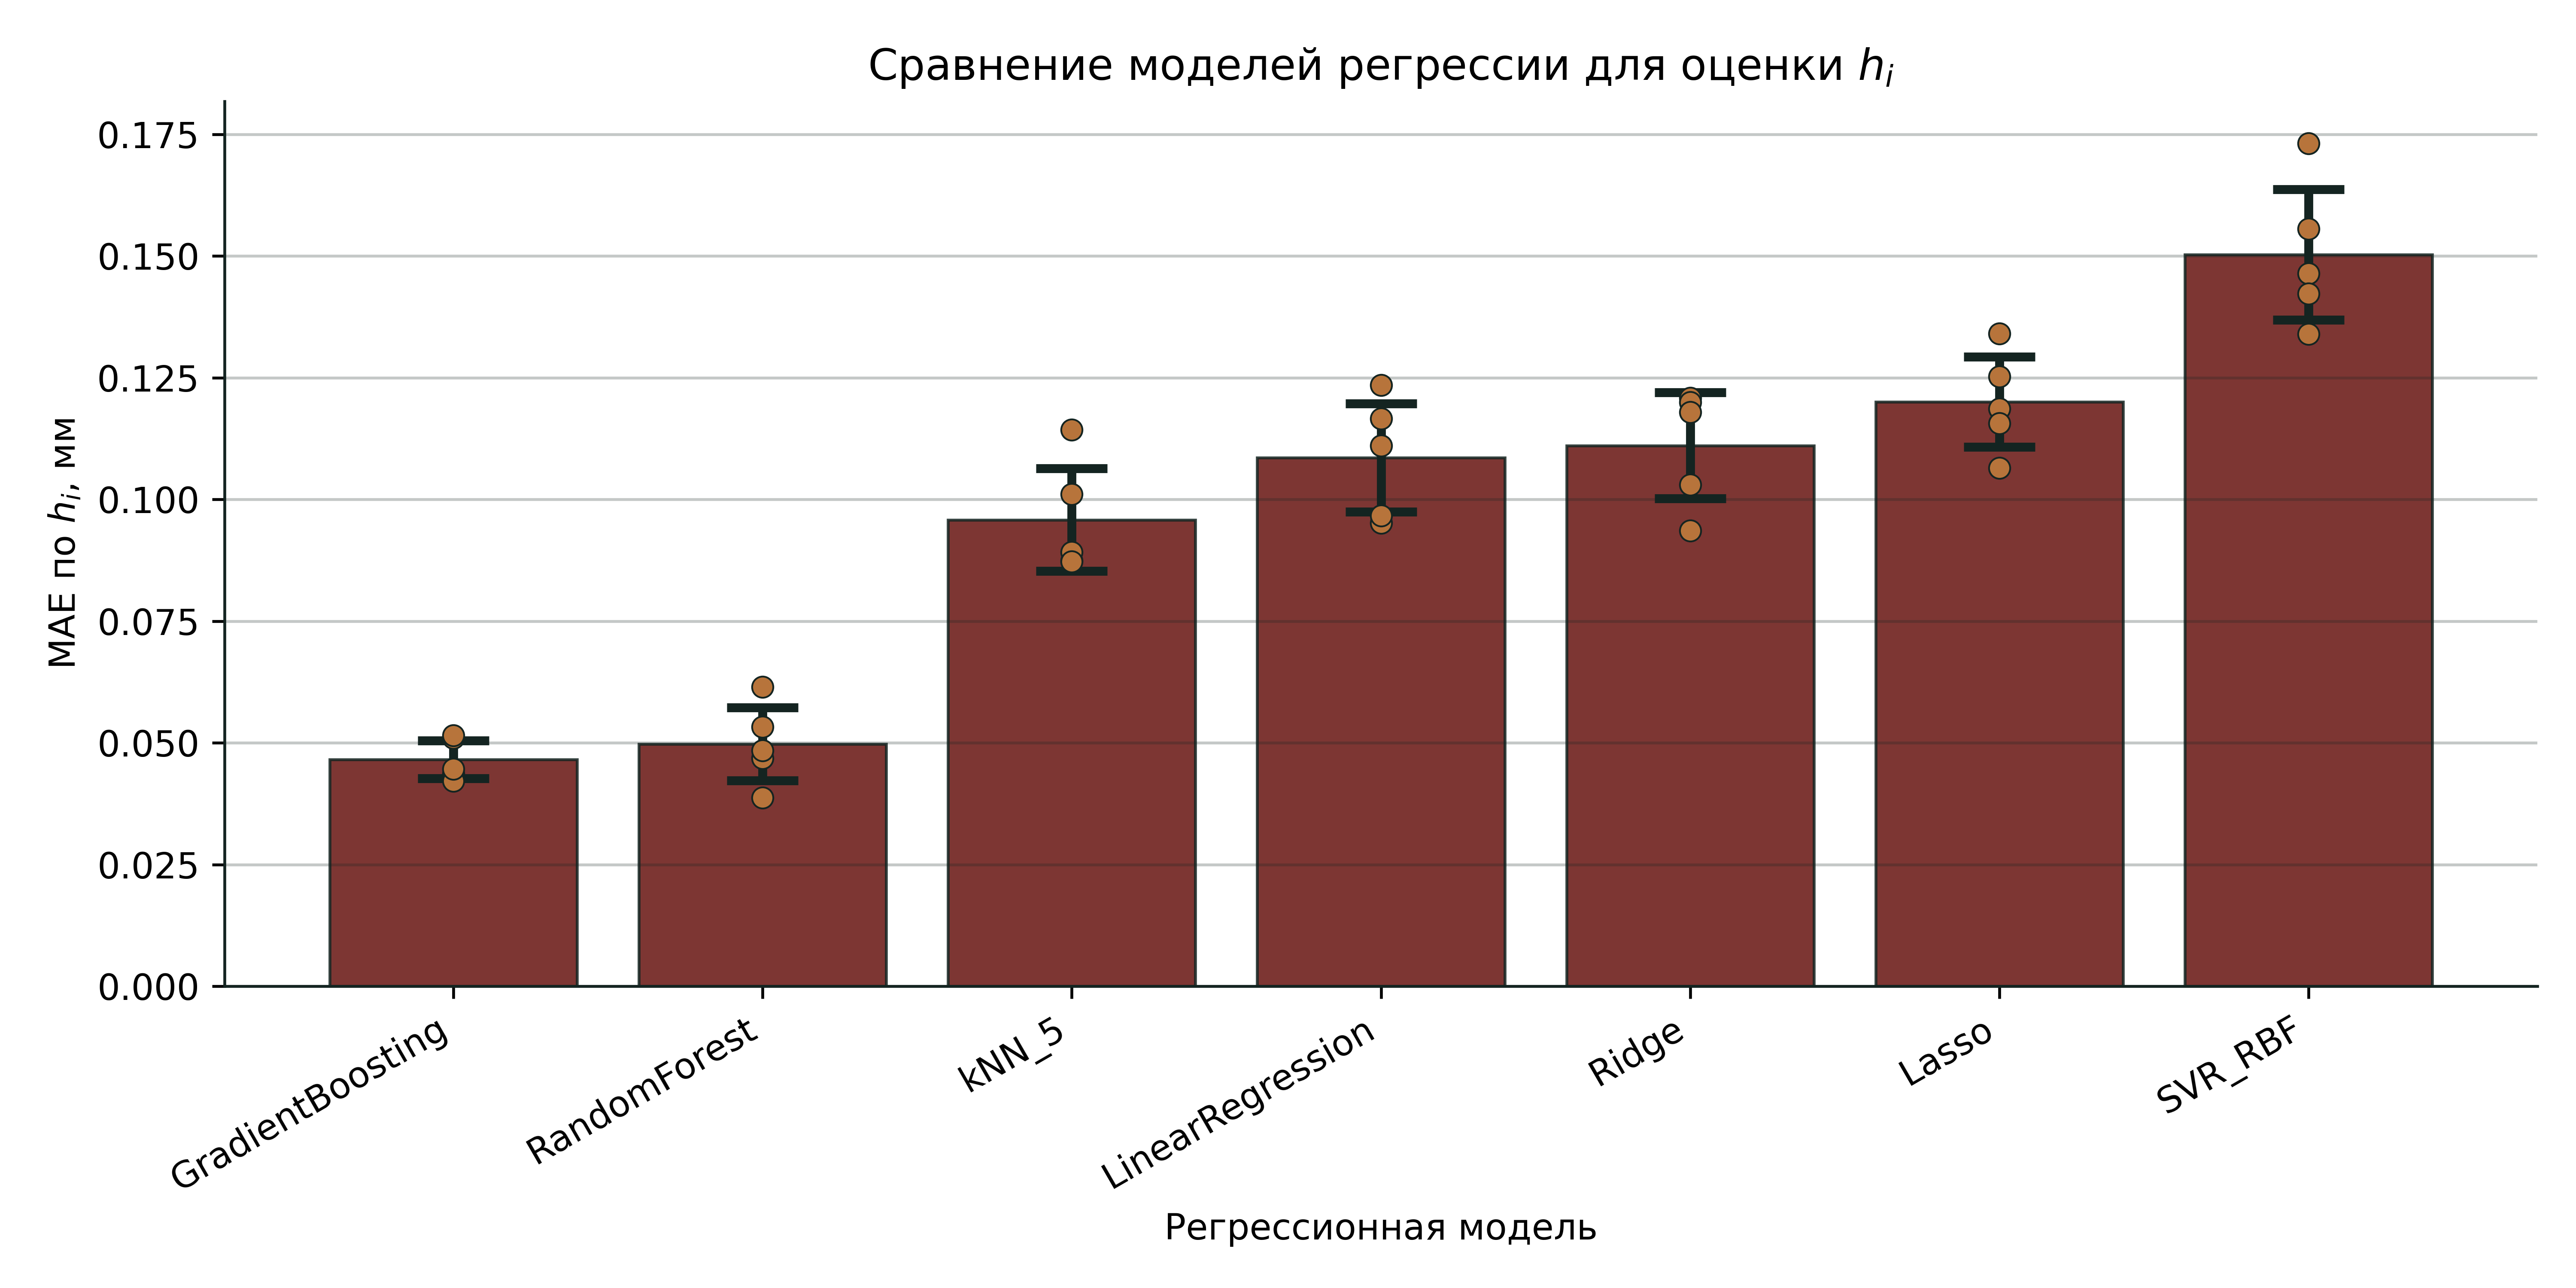
\includegraphics[width=0.86\textwidth]{figures/hi_regression_comparison.png}
    \caption{Сравнение регрессионных моделей при оценке \(h_i\) с использованием всех каналов фотодиодной системы}
    \label{fig:hi_regression_comparison_with_reflected}
\end{figure}

При использовании всех каналов наилучший результат был получен с использованием модели Gradient Boosting. Соответствующее распределение предсказанных значений \(h_i\) приведено на рис.~\ref{fig:hi_regression_with_reflected}.

\begin{figure}[H]
    \centering
    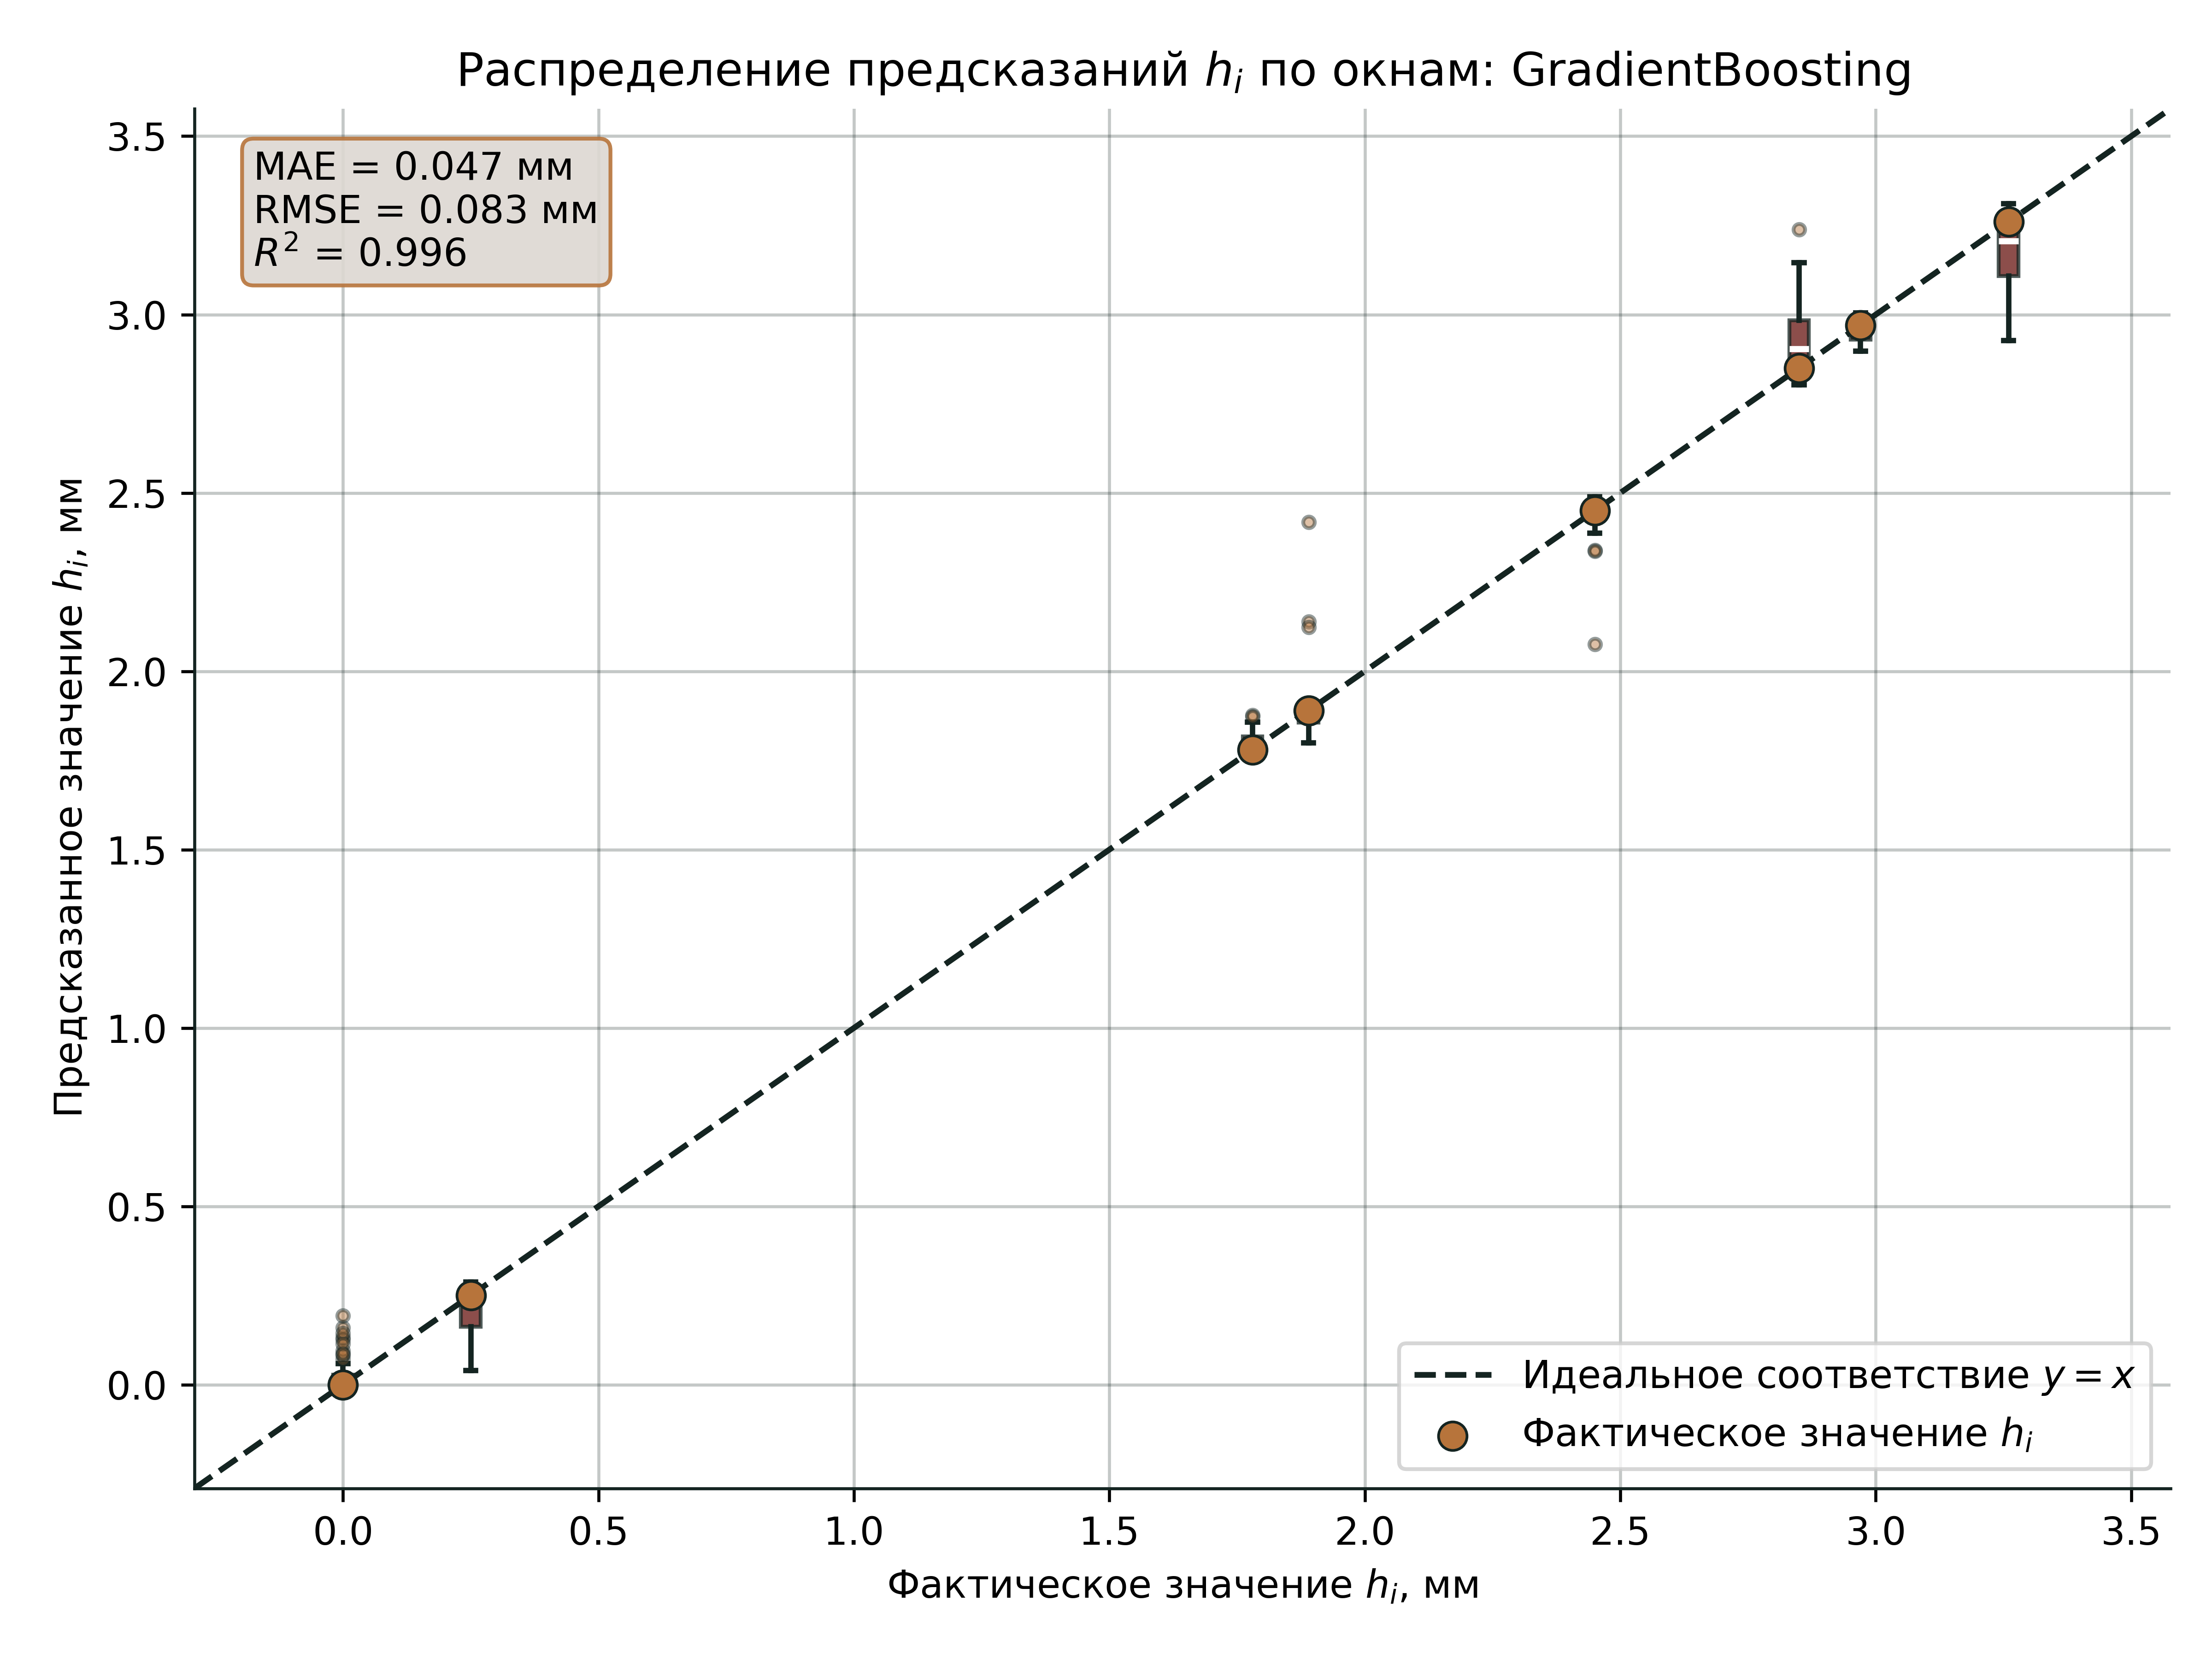
\includegraphics[width=0.78\textwidth]{figures/hi_true_vs_predicted.png}
    \caption{Распределение предсказанных значений \(h_i\) по окнам с использованием всех каналов фотодиодной системы}
    \label{fig:hi_regression_with_reflected}
\end{figure}

При использовании канала отражённого излучения средняя абсолютная ошибка составила 0.047~мм. Формально этот результат указывает на возможность достаточно точной количественной оценки \(h_i\). Однако его необходимо интерпретировать осторожно из-за структуры экспериментальной серии. В рассматриваемом наборе данных мощность лазерного излучения принимала только три дискретных значения: 1.5, 2.0 и 3.5~кВт. Канал отражённого излучения существенно связан с мощностью, поэтому его значения также фактически группируются в соответствии с этими тремя режимами.

При этом значения \(h_i\) в данной серии также связаны с мощностью: для режимов 1.5 и 2.0~кВт во всех измерениях наблюдался непровар, тогда как для режима 3.5~кВт в двух из трёх измерений непровар отсутствовал. В результате регрессионная модель при использовании канала отражённого излучения может опираться не столько на универсальные признаки формирования непровара, сколько на косвенное распознавание одного из трёх режимов мощности. Это создаёт риск переобучения на структуру  именно этой экспериментальной серии и может приводить к завышенной оценке точности.

Таким образом, количественная оценка \(h_i\) с использованием всех каналов является перспективной, но пока не может рассматриваться как полностью подтверждённая. Для её строгой проверки необходима более разнообразная экспериментальная выборка, в которой значения \(h_i\) изменяются при близких значениях мощности лазерного излучения.


\chapterconclusion

Была рассмотрена возможность оценки качества сварного соединения по сигналам коаксиальной фотодиодной системы. Основным объектом анализа являлось временное окно сигнала, что соответствует задаче контроля процесса в режиме, близком к реальному времени.

Качественная оценка была сформулирована как бинарная классификация по условию \(h_i = 0\) или \(h_i > 0\). Полученные результаты показали, что наличие непровара может быть определено по оконным признакам фотодиодных сигналов без использования канала отражённого излучения. Для модели LDA отсутствие непровара корректно определялось с вероятностью 85~\%, а наличие непровара 94~\%. Это подтверждает возможность оперативной качественной оценки качества шва.

Добавление канала отражённого излучения повышало качество моделей, однако этот результат требует осторожной интерпретации. В рассматриваемой серии этот канал связан с мощностью лазерного излучения, а величина \(h_i\) также изменяется совместно с мощностью. Поэтому качественный результат без канала отраженного излучения является более строгим с точки зрения проверки информативности собственно фотодиодных признаков относительно непровара.

Количественная оценка величины \(h_i\) была проверена с использованием регрессионных моделей. Без канала отражённого излучения наблюдался заметный разброс оконных предсказаний. При использовании всех каналов была получена малая средняя абсолютная ошибка, однако этот результат связан с особенностями структуры набора данных и требует подтверждения на расширенной экспериментальной серии.

Таким образом, по имеющимся данным возможно выполнять качественную оценку наличия непровара в режиме, близком к реальному времени. Количественная оценка величины непровара также является перспективной, но для её строгого обоснования требуется большее число экспериментов с более разнообразным сочетанием мощности лазерного излучения и величины \(h_i\).


\endinput
